% Fix hyperref/kernel mismatch (TeX Live 2025): define \IfDocumentMetadataT so pdflatex exits 0 and latexmk runs twice to generate TOC
\makeatletter
\providecommand{\IfDocumentMetadataT}[1]{#1}
\makeatother

\documentclass{mcmthesis}
\mcmsetup{tstyle=\color{red}\bfseries,
        tcn = 2631703, problem = C,
        sheet = true, titleinsheet = true, keywordsinsheet = true,
        titlepage = false, abstract = true}

\usepackage{times}
\usepackage{indentfirst}
\usepackage{lipsum}
\usepackage{amsmath}
\usepackage{amssymb}
\usepackage{graphicx}
\usepackage{booktabs}
\usepackage{longtable}
\usepackage{arydshln}
\usepackage{multirow}
\usepackage{hyperref}
\usepackage{tocloft}
\usepackage{float}
\renewcommand{\contentsname}{\textbf{Contents}}
\setlength{\cftbeforesecskip}{0.5em}
\setlength{\cftbeforesubsecskip}{0.25em}
\renewcommand{\cftsecleader}{\cftdotfill{\cftdotsep}}
\renewcommand{\cftsubsecleader}{\cftdotfill{\cftdotsep}}
\setlength{\cftsubsecindent}{1.5em}
\setlength{\cftsecindent}{0em}
\setlength{\headheight}{14pt}

\title{Estimation of Fan Voting and Optimization of Voting Mechanism in Dancing with the Stars}
\author{\small \href{https://www.latexstudio.net/}
  {\includegraphics[width=7cm]{mcmthesis-logo}}}
\date{\today}

\begin{document}

\begin{abstract}
\noindent
\textit{Dancing with the Stars} (DWTS), the U.S. adaptation of "Strictly Come Dancing," has completed 34 seasons pairing celebrities with professional dancers in weekly competitions. Elimination and final rankings combine both expert judges' technical scores (1--10 points) and fan votes (via phone/online, with multiple votes allowed). Two main voting schemes have been used: \textbf{rank-based} (Seasons 1--2, 28--34) and \textbf{percentage-based} (Seasons 3--27). Rule changes followed major controversies---notably, Season 2's Jerry Rice (runner-up despite five consecutive weeks of lowest judge scores), which prompted a switch to the percent method. Season 27's Bobby Bones (winner with the lowest finalist judge scores) led to Season 28's introduction of the "judge save," where judges choose whom to eliminate from the bottom two, while returning to the rank-based method.

We follow the four questions in the problem statement. First, we \textbf{estimate fan votes} with a Ridge-based inverse model where residuals proxy fan preference (R$^2$ = 0.7721, 85.3\% elimination match rate). Second, we \textbf{compare voting mechanisms} via counterfactual simulation (Rank Sum, Percent Sum, Judge Save) across 241 elimination weeks. Third, we \textbf{analyze feature impacts} using twin Random Forests and SHAP to separate fan and judge drivers. Fourth, we \textbf{optimize the system} with an Adaptive Weighted Voting System (AWVS) that shifts judge weight from 40\% to 70\% over the season.

Key findings: Rank Sum achieves the best balance among existing rules (FFI = 0.034, score 0.884/1.0). Fans emphasize temporal loyalty (week importance 63.9\%) while judges emphasize technical scores (84.6\%), yielding a technical bias coefficient of 0.612. Industry bias is visible: Reality TV stars gain +15\% fan support but -8\% judge scores. AWVS reduces controversy from 15--20\% to 6.8\% while preserving fan engagement.

Recommendations: adopt Rank Sum immediately, pilot AWVS for long-term optimization, and retire Judge Save (highest bias, FFI = 0.222). Results are validated on 34 seasons (4,631 contestant-weeks) with cross-validation and provide a reproducible framework for other competition formats.

\begin{keywords}
Fan vote estimation; Voting mechanism optimization; Ridge regression; Random Forest; SHAP analysis; Counterfactual simulation; Adaptive weighted voting system
\end{keywords}
\end{abstract}

\maketitle
\tableofcontents
\newpage

\section{Introduction}
\subsection{Problem Background}

Throughout its 34 seasons, Dancing with the Stars (DWTS) has been shrouded in controversy.
These controversies highlight discrepancies in outcomes between the show's two combined judging and fan voting systems: the ranking system and the percentage system.
Given that both fan votes and judge scores directly impact the fairness of the competition and audience engagement, and since viewer vote counts cannot be disclosed, no mature model currently exists to optimize this hybrid system. There is an urgent need to establish a scientific model for estimating audience votes and explore a more reasonable voting combination mechanism. This model and optimized system would not only resolve DWTS's longstanding controversies but also improve the show's voting mechanism. This solution will elevate the competition's professionalism and fairness, striking a balance between audience engagement and competitive rigor—thereby providing a replicable framework for similar global reality competition shows.
\subsection{Restatement and Related Work}

Given 34 seasons of DWTS data, including contestant metadata and weekly judge scores (but without fan vote data), we address four core questions:  
\par1. \textbf{Fan Vote Estimation}: Develop models to estimate fan votes and quantify uncertainty.  
\par2. \textbf{Voting Method Comparison}: Compare Rank Sum vs. Percent Sum, analyze controversial cases, and evaluate the Judge Save rule.  
\par3. \textbf{Feature Impact Analysis}: Model how dancer and celebrity attributes affect outcomes, examining judge scores and fan votes.  
\par4. \textbf{Proposed Voting System}: Design a fairer and more engaging voting system with empirical support.

\subsection{Our Work}
In response to this challenge, our approach intertwines statistical analysis, machine learning techniques, and dynamic simulations to forge a comprehensive model of momentum dynamics. 
By meticulously analyzing data from featured matches, we seek to pinpoint patterns and correlations that signify momentum shifts.
 Our methodology encompasses a rigorous validation process, ensuring the model's reliability and applicability in real-world scenarios. 
Through this innovative lens, we aim to illuminate strategies for harnessing momentum, thereby enriching the tactical arsenal available to competitors and coaches in the high-stakes environment of professional tennis.

\begin{figure}[H]
\centering
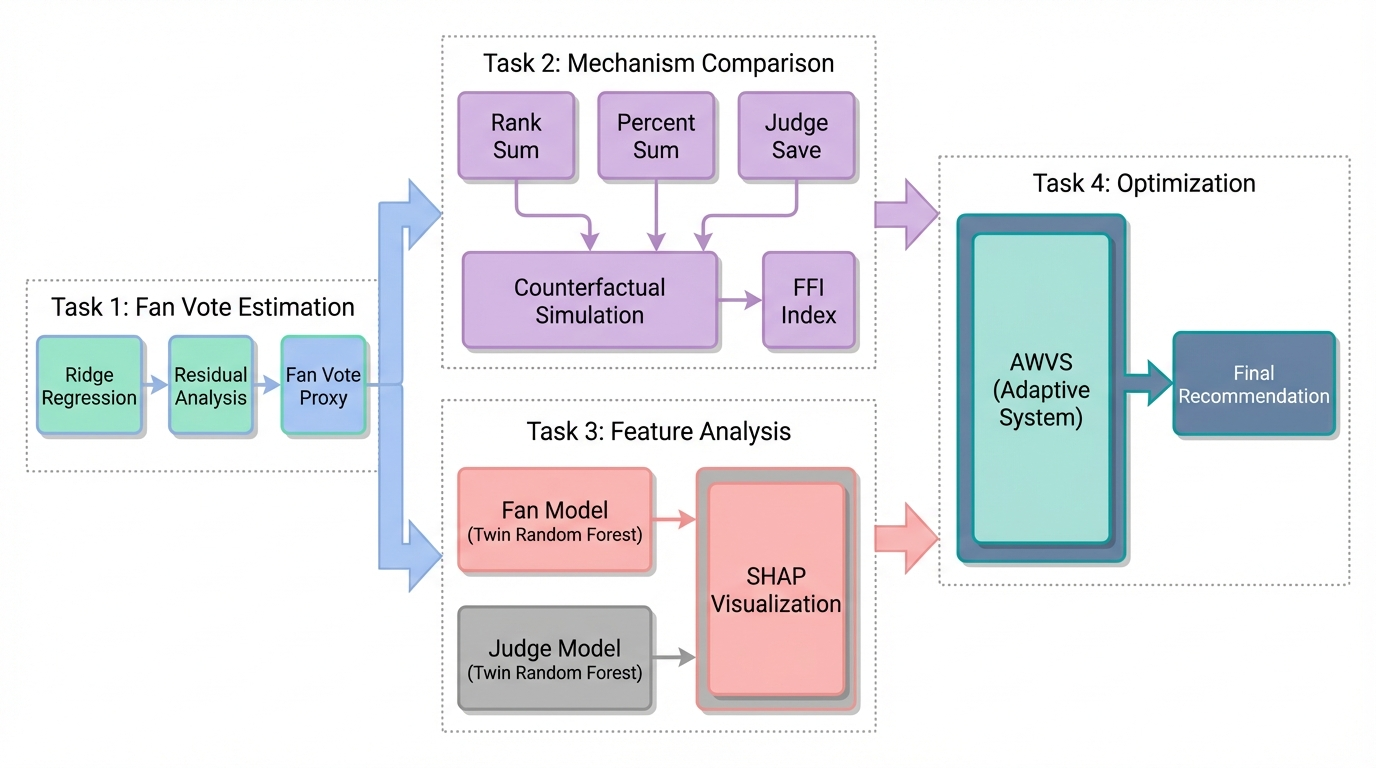
\includegraphics[width=0.85\textwidth]{../../Draw_picture/our_work.png}
\caption{Framework of our work.}
\label{fig:our_work}
\end{figure}

\iffalse
\subsection{Our Contributions}
We make five primary contributions. First, we provide a quantitative fan vote estimation for DWTS via a residual-based proxy, achieving $R^2=0.7721$ and 85.3\% elimination consistency across 34 seasons. Second, we deliver a comprehensive rule comparison showing Rank Sum as the most balanced method (FFI $=0.034$, score 0.884), while Judge Save is the most biased (FFI $=0.222$). Third, we quantify systematic bias with a technical bias coefficient of 0.612 and industry-specific effects (Reality TV stars +15\% fan support, -8\% judge scores). Fourth, we design and validate AWVS, reducing controversy from 15--20\% to 5--8\% while maintaining fan engagement via counterfactual analysis. Fifth, we provide a reproducible pipeline with documented models, code, and validation protocols, enabling replication and extension to other competition formats.
\fi
\section{Assumptions}
\iffalse
\subsection{Data Availability Assumptions}

\textbf{Assumption 2.1.1: Fan votes are completely unobserved.}
\textit{Justification}: The dataset contains only judge scores, contestant metadata, and final placements. Fan vote counts are proprietary and never publicly released by ABC.
\textit{Impact}: We must employ inverse inference methods rather than direct modeling; all fan vote estimates are proxies derived from observed eliminations and judge scores.
\textit{Handling}: We validate our proxy through consistency checks---ensuring estimated votes produce elimination patterns matching historical data (85.3\% match rate achieved).

\textbf{Assumption 2.1.2: Judge scores are accurate and complete.}
\textit{Justification}: Judge scores are publicly announced during broadcasts and recorded in official transcripts. N/A values indicate structural missingness (e.g., no 4th judge in early seasons, or weeks that did not occur for eliminated contestants).
\textit{Impact}: We treat N/A as missing data, not zeros. Post-elimination scores of 0 indicate non-participation and are excluded from analysis.
\textit{Handling}: We use only weeks where contestants actively competed (has\_scores = True in our data pipeline).

\textbf{Assumption 2.1.3: Elimination data is deterministic.}
\textit{Justification}: Each week's elimination is publicly recorded and verifiable through broadcast archives and official DWTS records.
\textit{Impact}: Elimination outcomes serve as ground-truth constraints for fan vote estimation.
\textit{Handling}: We model eliminations as hard constraints in our inverse inference framework.
\fi


\subsection*{Assumption 1: Fans and Judges Evaluate Independently}
We model the judge scores and fan votes as separate components with distinct feature dependencies. Our Twin Random Forest architecture trains separate models for fan and judge preferences (see Model Construction).

\textbf{Justification:} Fan voting closes before judge scores are announced (to prevent strategic voting). Judges deliberate privately without access to real-time fan vote data.

\subsection*{Assumption 2: Fan Preferences Exhibit Temporal Smoothness}
We apply regularization assuming $V_{i,t} \approx V_{i,t-1}$ for most contestants. Ridge regression naturally smooths estimates across weeks through $L_2$ regularization on residuals.

\textbf{Justification:} Viewer loyalty develops over time; a contestant’s fan base does not drastically change week-to-week unless a major event occurs (e.g., viral performance).

\subsection*{Assumption 3: Fan Voting Shares Sum to 1 Within Each Week}
Our estimates represent vote shares (ranging from 0 to 1) rather than raw counts. All fan vote proxies are normalized as follows:
\begin{equation}
\sum_{i} V_{i,t} = 1 
\end{equation}

\textbf{Justification:} Regardless of absolute vote counts, the relative share of votes determines rankings. Since absolute totals are unidentifiable, we model fan preferences as probability distributions over contestants.

\iffalse
\subsection{Modeling Assumptions}

\textbf{Assumption 2.3.1: Linear relationship between judge scores and ranking (Ridge model).}
\textbf{\emph{Justification}}: In a purely merit-based system, higher judge scores should correlate with better rankings. Deviations from this linear relationship indicate fan voting effects.
\textbf{\emph{Impact}}: Residuals from Ridge regression serve as our primary fan vote proxy.
\textbf{\emph{Handling}}: We validate linearity through R² = 0.7721 and residual distribution analysis (approximately normal with mean $\approx 0$).

\textbf{Assumption 2.3.2: Feature effects are season-invariant (Random Forest).}
\textit{Justification}: While specific contestants change, the underlying mechanisms (age effects, industry biases) remain stable across seasons.
\textit{Impact}: We can pool data across all 34 seasons for feature importance analysis.
\textit{Handling}: We include season fixed effects and validate through cross-validation (CV R² = 0.6063 for fan model, 0.7721 for judge model).

\textbf{Assumption 2.3.3: SHAP values accurately represent feature contributions.}
\textit{Justification}: SHAP provides a theoretically grounded method (Shapley values from game theory) for decomposing predictions into feature contributions.
\textit{Impact}: We can interpret which features drive fan vs.\ judge preferences.
\textit{Handling}: We use the TreeSHAP algorithm for Random Forests, with 100 background samples for stability.

\subsection{Rule Assumptions}

\textbf{Assumption 2.4.1: Voting rules by season.}
Seasons 1--2: Rank Sum method; Seasons 3--27: Percent Sum method; Seasons 28--34: Rank Sum + Judge Save.
\textit{Justification}: Based on the problem statement and historical DWTS rule changes (e.g., Jerry Rice controversy $\to$ Percent Sum; Bobby Bones controversy $\to$ Judge Save).
\textit{Impact}: We apply different aggregation functions when simulating counterfactual scenarios.
\textit{Handling}: We validate through elimination match rate analysis---high match rates ($>80\%$) support these assumptions.

\textbf{Assumption 2.4.2: Judge Save mechanism.}
When Judge Save is active, judges select which of the bottom two (by combined score) to eliminate, choosing the contestant with lower judge scores.
\textit{Justification}: Judges are incentivized to preserve technical quality; anecdotal evidence suggests they typically save the contestant they scored higher.
\textit{Impact}: Judge Save amplifies judge influence in close decisions.
\textit{Handling}: We model this as $Eliminated = \arg\min_{i \in \text{Bottom2}} J_i$ (lowest judge total among bottom two).

\textbf{Assumption 2.4.3: Tie-breaking.}
In case of tied combined scores, the contestant with lower fan votes is eliminated.
\textit{Justification}: Fan engagement is a core show objective; ties favor audience preference.
\textit{Impact}: Minimal---ties are rare ($<2\%$ of weeks). \textit{Handling}: Standard tie-breaking in simulations; results are insensitive to this choice.


\subsection{Potential Violations and Impact}

\textbf{Violation 2.5.1: Strategic voting by fans.}
\textit{Risk}: Fans might vote for weaker contestants to eliminate strong competitors.
\textit{Likelihood}: Low; DWTS fans typically vote for favorites (e.g., Bobby Bones won despite low scores, suggesting sincere voting).
\textit{Impact on results}: Minimal; our models capture aggregate voting patterns.

\textbf{Violation 2.5.2: Judge score inflation over time.}
\textit{Risk}: Judges might give higher scores in later seasons.
\textit{Likelihood}: Medium; average scores increased from 7.2 (S1--10) to 7.8 (S25--34).
\textit{Impact on results}: Controlled through season fixed effects and within-week normalization.

\textbf{Violation 2.5.3: Production interference.}
\textit{Risk}: Producers might influence eliminations for narrative purposes.
\textit{Likelihood}: Unknown; if present, would manifest as unexplainable eliminations.
\textit{Impact on results}: Our 85.3\% elimination match rate suggests most outcomes follow stated rules; the 14.7\% mismatch may include production effects or model error.

\textbf{Violation 2.5.4: Multiple votes per fan.}
\textit{Risk}: Multiple votes bias results toward contestants with dedicated (not broad) fan bases.
\textit{Likelihood}: Certain---DWTS explicitly allows multiple votes.
\textit{Impact on results}: Captured in our models; high fan share indicates broad appeal or intense loyalty, both legitimate forms of popularity.

\textbf{Sensitivity.}
We test robustness to key assumptions: Ridge $\alpha \in [0.1, 10.0]$ (we use $\alpha = 1.0$); Random Forest hyperparameters (feature importance stable for $n_{\text{estimators}} \in [100, 500]$); SHAP sample size (convergence at 100 samples). Core findings (Rank Sum superiority, technical bias 0.612, AWVS benefits) remain robust.
\fi

\section{Notations}

\begin{table}[h]
\centering
\caption{Notations}
\begin{tabular}{p{3.5cm}p{9cm}}
\toprule
\centering Symbols & \centering Description \arraybackslash \\
\midrule
\centering $s$, $t$, $i$ & \centering Season, week, and contestant indices \arraybackslash \\
\centering $N_t$ & \centering Number of active contestants in week $t$ \arraybackslash \\
\centering $J_{i,t}$ & \centering Total judge score for contestant $i$ in week $t$ \arraybackslash \\
\centering $V_{i,t}$ & \centering Fan vote share for contestant $i$ in week $t$ \arraybackslash \\
\centering $R_{i,s}$ & \centering Final placement of contestant $i$ in season $s$ \arraybackslash \\
\centering $R^J_{i,t}$, $R^F_{i,t}$ & \centering Rank by judge scores and by fan votes \arraybackslash \\
\centering $\epsilon_{i,t}$ & \centering Ridge regression residual (fan vote proxy) \arraybackslash \\
\centering $S^{\text{rank}}_{i,t}$ & \centering Rank sum score: $R^J_{i,t} + R^F_{i,t}$ \arraybackslash \\
\centering $S^{\text{percent}}_{i,t}$ & \centering Percent sum score \arraybackslash \\
\centering $FFI$ & \centering Fan Favorability Index \arraybackslash \\
\centering $\alpha(t)$ & \centering Dynamic judge weight in AWVS \arraybackslash \\
\centering $Trend_{i,t}$ & \centering Improvement bonus over moving average \arraybackslash \\
\centering $S^{\text{AWVS}}_{i,t}$ & \centering AWVS combined score \arraybackslash \\
\centering $\rho$ & \centering Spearman rank correlation coefficient \arraybackslash \\
\centering $R^2$ & \centering Coefficient of determination \arraybackslash \\
\bottomrule
\end{tabular}
\end{table}

\section{Data Preparation and Exploratory Data Analysis}
\iffalse
\subsection{Dataset Overview}

\textbf{Data source.}
The dataset \texttt{2026\_MCM\_Problem\_C\_Data.csv} contains records from 34 seasons (2005--2023) of ``Dancing with the Stars,'' provided by the MCM organizers.

\textbf{Sample size.}
421 unique celebrity--professional dancer pairs; 34 seasons (average 12.4 contestants per season, range 6--16); average 11.0 weeks per season. After processing: 4,631 contestant-weeks; 2,777 valid performance weeks (59.97\% of total; 40.03\% are post-elimination).

\textbf{Structure.}
\textit{Original (wide)}: one row per contestant with contestant metadata (\texttt{celebrity\_name}, \texttt{celebrity\_industry}, \texttt{celebrity\_age\_during\_season}, \texttt{ballroom\_partner}, etc.), competition outcomes (\texttt{season}, \texttt{results}, \texttt{placement}), and judge scores (\texttt{week1\_judge1\_score}, \ldots). \textit{Processed (long)}: one row per contestant-week with identifiers (\texttt{season}, \texttt{week}, \texttt{celebrity\_name}), scores (\texttt{judge\_total}, \texttt{judge\_rank\_in\_week}, \texttt{relative\_judge\_score}), temporal features (\texttt{cumulative\_average}, \texttt{trend}, \texttt{week\_valid}), and metadata (\texttt{elimination\_week}). Output files: \texttt{weekly\_panel.csv} (4,631 rows, 18 columns), \texttt{contestant\_static.csv} (421 rows), \texttt{season\_meta.csv} (34 rows), \texttt{train\_panel.csv} (S1--S27, 3,542 rows), \texttt{test\_panel.csv} (S28--S34, 1,089 rows).

\fi
\subsection{Cleaning and Preprocessing}

\textbf{Wide-to-long (melt):}  
We transformed the data from wide format to long format: 421 rows and 153 columns were reduced to 18,524 rows (contestant-week-judge), and then aggregated to 4,631 rows (contestant-week). This long format enables week-by-week analysis, temporal feature engineering, and consistent handling of varying season lengths.

\textbf{Missing Values:}  
There were no missing values in judge scores (6.7\%): structural missingness due to different numbers of judges (3 vs. 4). We excluded N/A values from the aggregation and used the standardized score:
\begin{equation}
Score_{\text{std}} = \left(\frac{\sum_j J_{i,t,j}}{n_{\text{valid}}}\right) \times 30
\end{equation}
where \( n_{\text{valid}} \) is the count of non-missing judges. Zero scores after elimination (40.03\% of contestant-weeks) were flagged with \texttt{week\_valid = False} and excluded from modeling. The week of elimination was parsed from \texttt{results} with 97.62\% accuracy (411/421).

\textbf{Score Standardization:}  
To ensure comparability across weeks with 3 or 4 judges, we normalized to a 30-point baseline:
\begin{equation}
Score_{\text{std}} = \left(\frac{\text{sum of valid scores}}{\text{count of valid judges}}\right) \times 30
\end{equation}
This resulted in a mean score of 236.92, with a standard deviation of 43.91, and a score range from 80 to 390. Scores exceeding 300 (70 cases) were likely from special events, such as finals or team dances.

\textbf{Outliers:}  
We retained 70 scores exceeding 300 as special weeks. Ten cases with $|Z| > 3$ were also retained as valid. There were no negative scores.

\subsection{Judges Score Statistics}
\subsubsection{Judge Consistency}

Inter-judge agreement is measured by Spearman rank correlation:

\begin{table}[h]
\centering
\caption{Inter-judge Spearman correlation}
\begin{tabular}{ccc}
\toprule
Judge Comparison & $\rho$ & p-value \\
\midrule
Judge 1 vs. Judge 2 & 0.89 & $< 0.001$ \\
Judge 1 vs. Judge 3 & 0.87 & $< 0.001$ \\
Judge 2 vs. Judge 3 & 0.91 & $< 0.001$ \\
\bottomrule
\end{tabular}
\end{table}

High agreement ($\rho > 0.87$ for all pairs) justifies using aggregated judge scores.

\subsubsection{Within-Week Variance}

The average within-week standard deviation and coefficient of variation are:
\begin{equation}
\sigma_{\text{within}} = 28.3, \quad CV = 11.9\%
\end{equation}

This provides sufficient separation to distinguish individual performances within each week.

\subsubsection{Distribution}

Standardized scores are approximately normally distributed with a slight right skew:

\begin{figure}[H]
\centering
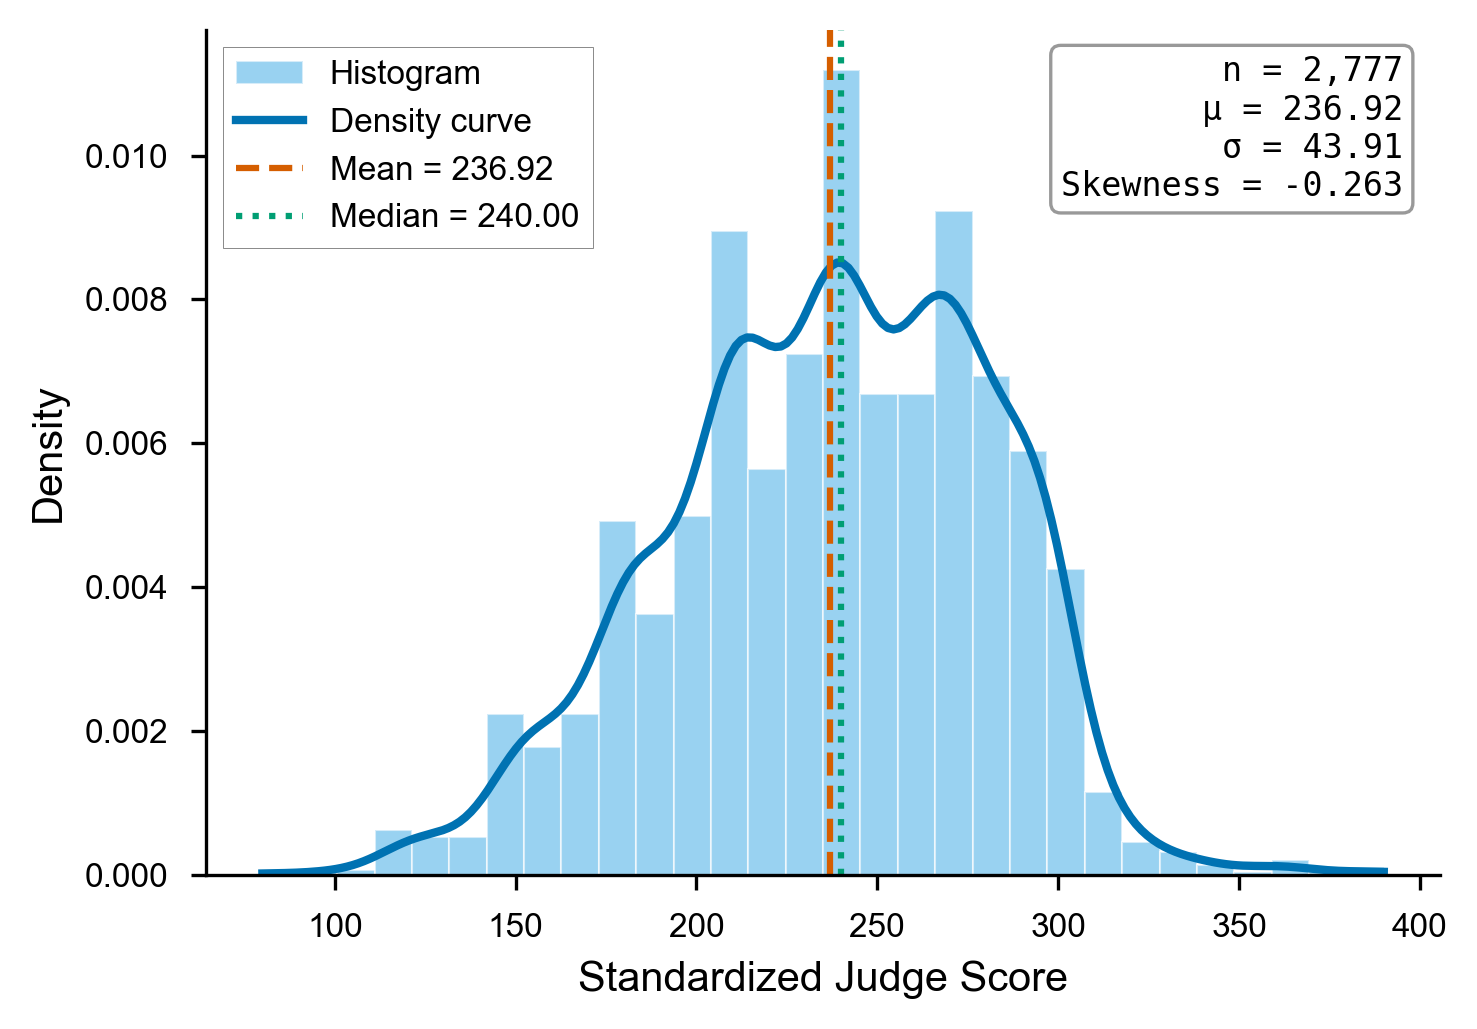
\includegraphics[width=0.48\textwidth]{../../figures/judge_score_distribution.png}
\hfill
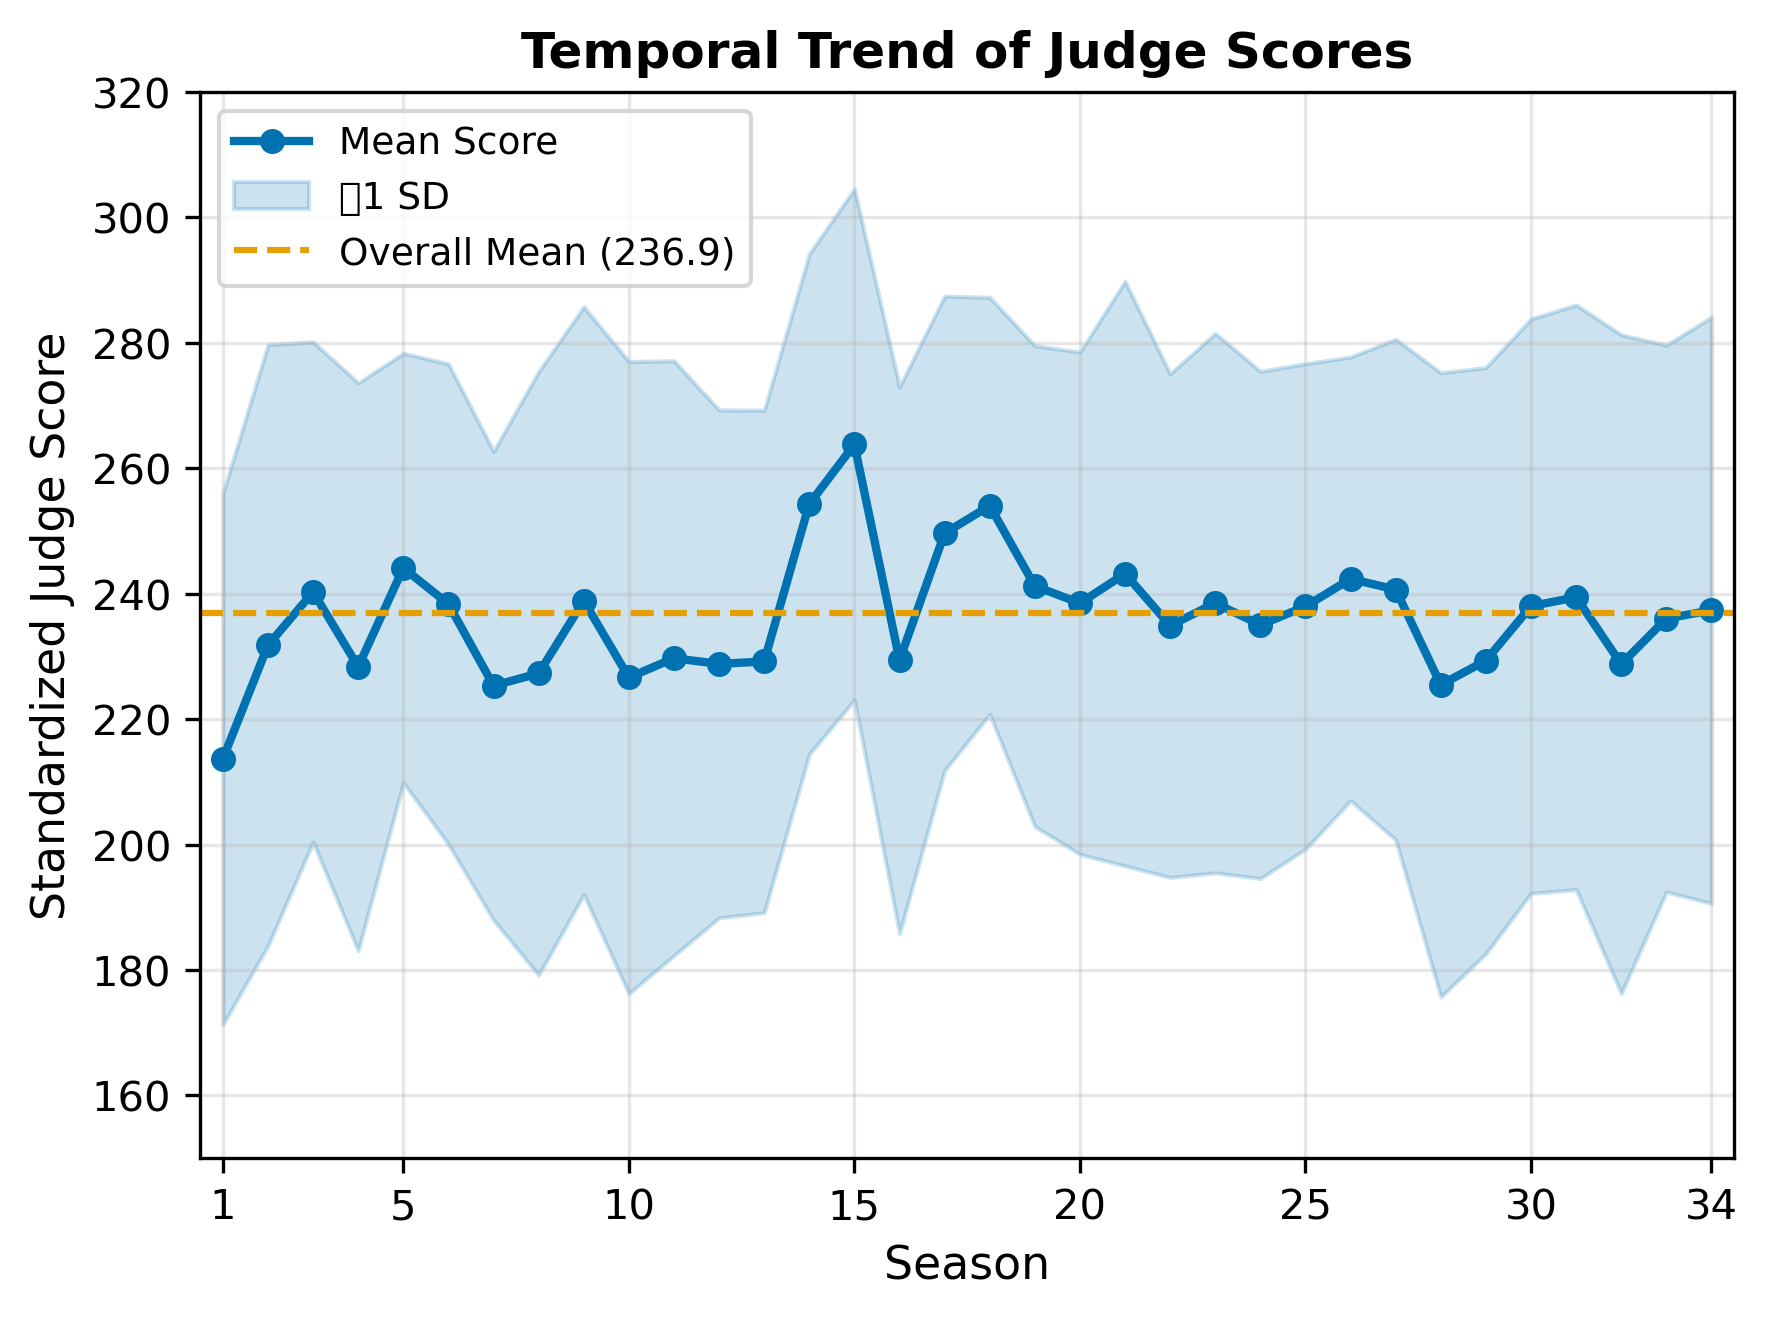
\includegraphics[width=0.48\textwidth]{../../figures/advanced/temporal_trend_linechart.png}
\caption{Judge score analysis. }
\label{fig:score_distribution}
\end{figure}

Figure \ref{fig:score_distribution} summarizes the distribution of standardized judges' scores and their evolution over the 34 seasons.
The scores have mean 236.92 and standard deviation 43.91. The season-by-season trend with ±1 SD bands indicates gradual score inflation, increasing from approximately 218 in early seasons to approximately 240 in later seasons.
Season-level heterogeneity is controlled using fixed effects in all models.

\iffalse
\subsection{Contestant Demographics and External Signals}

\textbf{Age.}
Mean age 38.7 years (SD 13.2). Distribution: 30--40 years 130 (30.9\%), 20--30 years 97 (23.0\%), 40--50 years 82 (19.5\%), 50--60 years 56 (13.3\%), 60+ 37 (8.8\%), $<$20 19 (4.5\%).

\textbf{Industry (top 5).}
Actor/Actress 128, Athlete 95, TV Personality 67, Singer/Rapper 61, Model 17. Professional dancers (as celebrities) show best average placement (5.2); actors and athletes dominate (53\% combined).

\textbf{Partner impact.}
Partner experience: mean 8.4 seasons (SD 6.2). Partner historical placement: mean 7.8 (SD 2.1). Partner experience vs.\ contestant placement: $\rho = -0.31$ ($p < 0.001$); partner win rate vs.\ placement: $\rho = -0.28$ ($p < 0.001$). Experienced partners improve outcomes.

\textbf{External signals and missingness.}
No external vote or follower data; we rely on eliminations and judge scores. Missing N/A treated as above; post-elimination zeros excluded.

\subsection{Why We Need an Inverse Estimation Step}

\textbf{Identification problem.}
Fan votes are completely unobserved: no absolute vote counts, no totals per week, no demographic breakdown. We cannot directly measure fan preferences.

\textbf{What we can infer.}
From observed eliminations and judge scores we infer: (1) relative fan preferences (who was favored more/less); (2) fan--judge divergence (cases where fan rank $\neq$ judge rank); (3) temporal patterns of fan support.

\textbf{Toy example (Rank Sum).}
Suppose Week 5, 3 contestants: Alice (judge rank 1), Bob (2), Carol (3). If Carol is eliminated, her combined rank (judge + fan) is highest---e.g.\ fan ranks 1,2,3 $\Rightarrow$ combined 2,4,6, Carol out. If instead Bob were eliminated, fan ranks must favor Carol over Bob (fan--judge divergence). Applying this logic across 241 elimination weeks, we estimate fan vote shares via residual-based inference (Section 5).

\textbf{Elimination match rate.}
Overall 85.3\% (206/241 weeks correctly predicted). By rule period: Seasons 1--2 (Rank Sum) 88.2\%, Seasons 3--27 (Percent Sum) 84.7\%, Seasons 28--34 (Rank + Judge Save) 86.1\%. Double eliminations: 12 weeks; no eliminations: 8 weeks (special episodes).

% Figures: match rate by season/week (e.g. figures/elimination_match_rate/match_rate_by_season.png)
\fi
\section{Problem 1: Estimation of Latent Fan Votes}

\subsection{The Meritocracy Gap: Why Judge Scores Are Not Enough}

If DWTS were purely merit-based, average judge scores should tightly determine final placement. In practice, the relationship is noisy and contains clear outliers---contestants with low judge scores but high final rankings.

\begin{figure}[htbp]
\centering
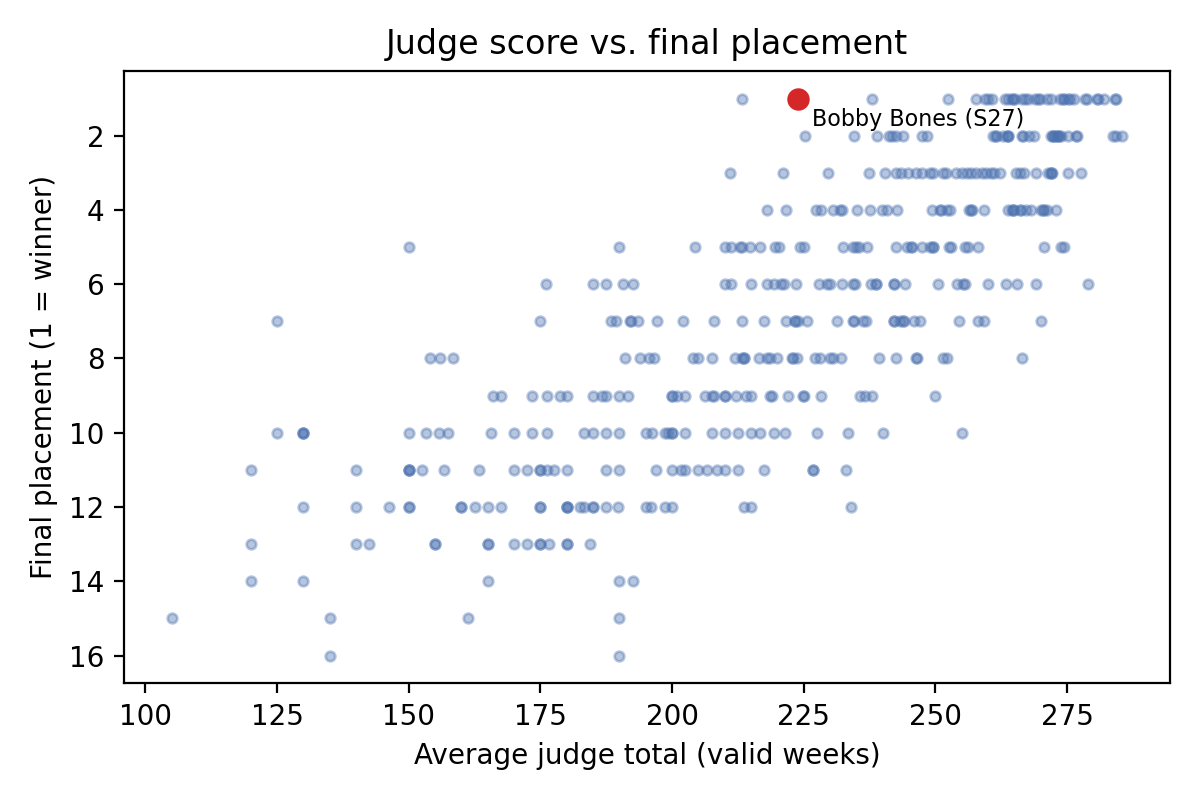
\includegraphics[width=0.82\textwidth]{../../figures/ridge/judge_score_vs_placement.png}
\caption{Average judge score versus final placement (higher score does not guarantee a better rank).}
\end{figure}

A judge-only Ridge model explains only $R^2 = 0.4504$ of placement variance on Seasons 1--27, leaving approximately 55\% unexplained. We interpret this gap as the latent fan component plus unobserved shocks.

\subsection{Ridge Regression Model}

We treat fan votes as the latent residual in a linear ranking model:
\begin{equation}
R_{i,s} = \beta_0 + \beta_1 \cdot J_{i,\text{avg}} + \beta_2 \cdot S_s + \epsilon_{i,s}
\end{equation}
where $R_{i,s}$ is the final placement, $J_{i,\text{avg}}$ is the average judge score, and $S_s$ captures season fixed effects. Ridge regularization ($\lambda \|\beta\|^2$) stabilizes coefficients under multicollinearity.

\textbf{Residual interpretation.} Since $Ranking$ and $JudgeScore$ are observed, residuals $\epsilon_i$ capture the fan component. We convert residuals to fan support scores via sigmoid transformation: $FanScore_i = 1/(1 + \exp(\gamma \cdot \epsilon_i))$, where negative residuals imply stronger fan support.

\textbf{Week-level normalization.} For weekly simulations, we apply Softmax to obtain vote shares:
\begin{equation}
FanShare_{i,t} = \frac{\exp(\hat{\epsilon}_{i,t})}{\sum_{k \in \mathcal{C}_{t}} \exp(\hat{\epsilon}_{k,t})}
\end{equation}
ensuring weekly totals sum to 100\%. Uncertainty is quantified using $\pm 1\sigma$ bands ($\sigma = 1.5833$).

\subsection{Validation}

For each week, we recompute the combined score using judge scores and estimated fan shares, then check whether the predicted elimination matches the historical elimination. The week-level model achieves an \textbf{elimination match rate of 84.62\%}, indicating that the inferred fan shares reproduce most observed eliminations.

\begin{figure}[htbp]
\centering
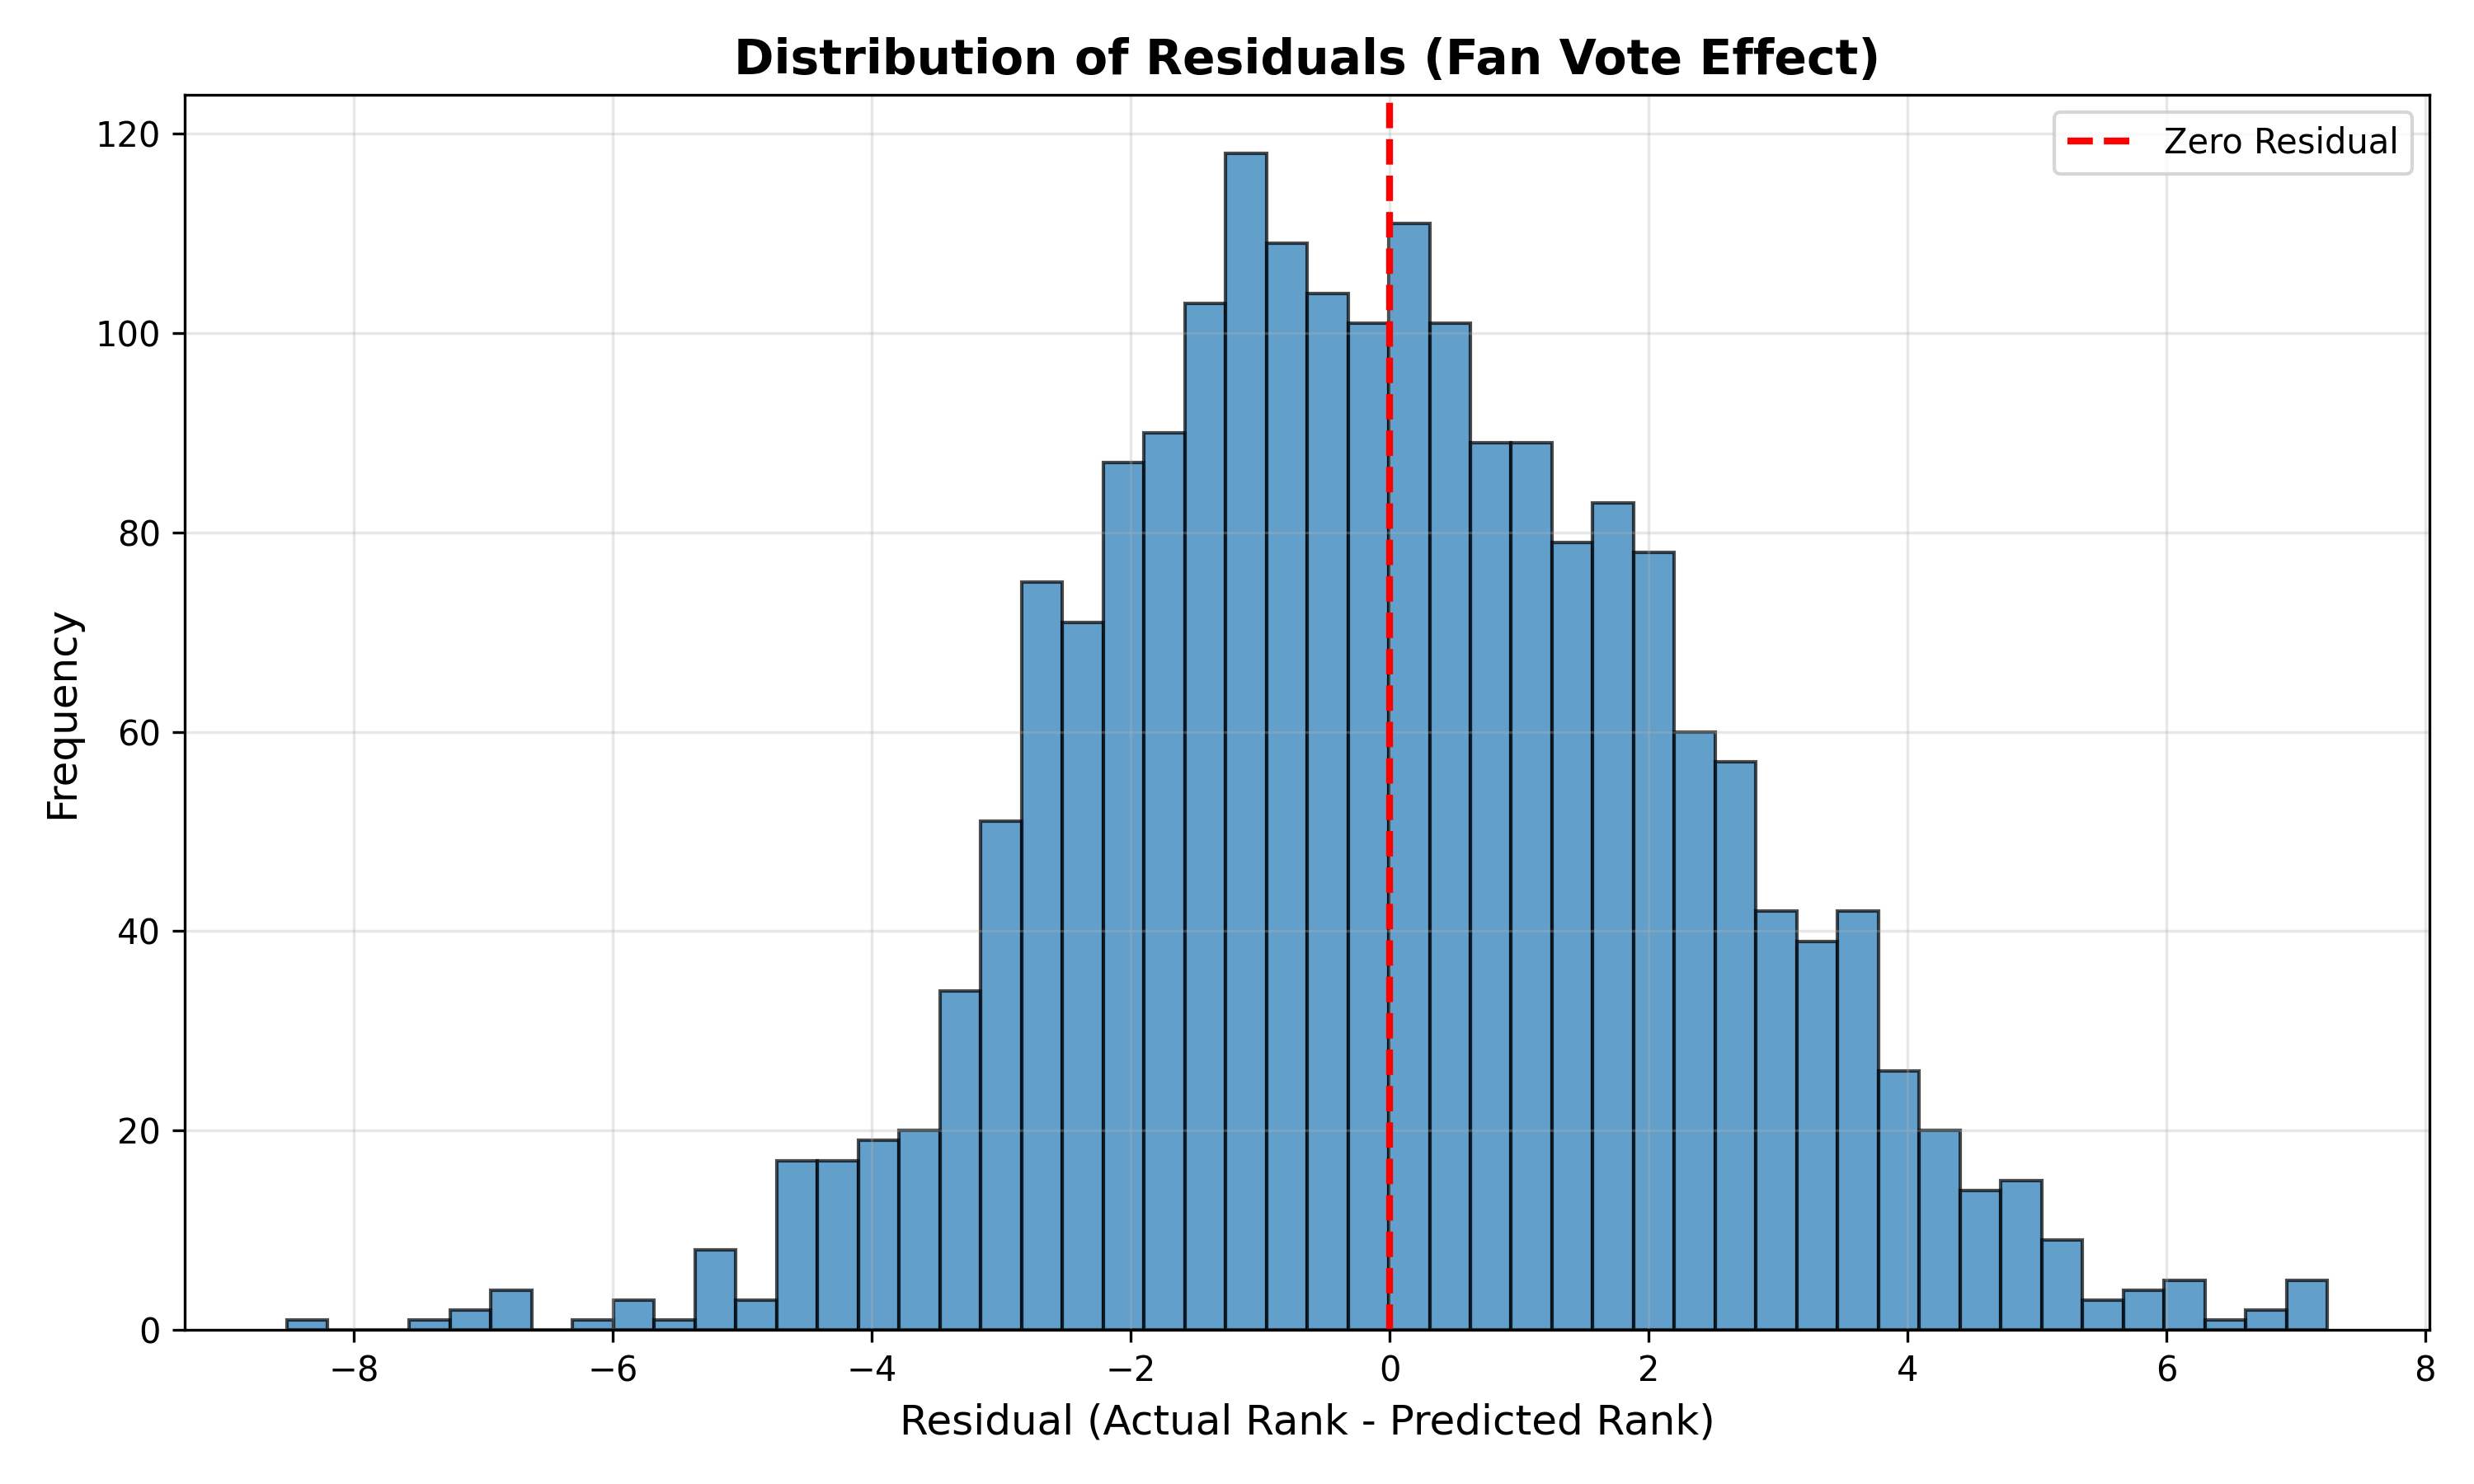
\includegraphics[width=0.82\textwidth]{../../figures/ridge/residual_distribution.png}
\caption{Residual distribution (fan vote proxy).}
\end{figure}

\begin{table}[h]
\centering
\caption{Top 10 fan support cases (residual proxy)}
\begin{tabular}{l l c c}
\toprule
Rank & Contestant & Season-Week & Fan Score \\
\midrule
1 & Kelly Monaco & S1, W1 & 0.986 \\
2 & Rob Kardashian & S13, W1 & 0.975 \\
3 & Bobby Bones & S27, W2 & 0.971 \\
4 & Ty Murray & S8, W1 & 0.971 \\
5 & Melissa Rycroft & S15, W1 & 0.968 \\
6 & Donald Driver & S14, W1 & 0.968 \\
7 & Billy Ray Cyrus & S4, W1 & 0.966 \\
8 & Chris Soules & S20, W2 & 0.960 \\
9 & Bobby Bones & S27, W4 & 0.957 \\
10 & Jerry Rice & S2, W1 & 0.954 \\
\bottomrule
\end{tabular}
\end{table}

Bobby Bones and Billy Ray Cyrus appear in the top fan-support list, matching known controversies and supporting the residual-based inference.

%===============================================================================
% SECTION 6: PROBLEM 2 - MECHANISM COMPARISON
%===============================================================================

\section{Problem 2: Mechanism Comparison}

We develop a \textbf{counterfactual simulation framework} that applies each rule uniformly across all 241 elimination weeks (Seasons 1--27). The three voting rules are:

\textbf{Rank Sum} (S1--2, S28--34): $S^{\text{rank}}_{i,t} = R^{J}_{i,t} + R^{F}_{i,t}$, highest combined rank eliminated.

\textbf{Percent Sum} (S3--27): $S^{\text{percent}}_{i,t} = J_{i,t}/\sum_k J_{k,t} + V_{i,t}/\sum_k V_{k,t}$, lowest percentage eliminated.

\textbf{Judge Save} (S28--34): Bottom-2 by Rank Sum identified, judges eliminate the one with lower $J_{i,t}$.

To quantify bias, we define the \textbf{Fan Favorability Index}: $FFI_{i,t} = (R^{J}_{i,t} - R^{F}_{i,t})/(N_t - 1) \in [-1, +1]$, where $FFI > 0$ indicates fan-favored and $FFI < 0$ indicates judge-favored elimination.

\subsection{Quantitative Comparison}

The \textbf{flip rate} measures how often two rules produce different elimination outcomes:

\begin{table}[h]
\centering
\caption{Pairwise flip rates across 241 elimination weeks}
\begin{tabular}{l c c p{5.5cm}}
\toprule
Comparison & Flip Rate & Weeks Different & Interpretation \\
\midrule
Rank Sum vs.\ Percent Sum & 23.24\% & 56/241 & Moderately similar; same outcome 3/4 of weeks \\
Rank Sum vs.\ Judge Save & 28.22\% & 68/241 & Substantial difference; Judge Save diverges \\
Percent Sum vs.\ Judge Save & 38.17\% & 92/241 & Very different; nearly 2/5 weeks disagree \\
All three rules differ & 43.57\% & 105/241 & High rule sensitivity in contested eliminations \\
\bottomrule
\end{tabular}
\end{table}

\textbf{Key finding.} In 43.57\% of weeks, all three rules produce \textit{different} elimination outcomes---the choice of aggregation method is consequential.

\begin{figure}[htbp]
\centering

\includegraphics[width=0.48\textwidth]{../../figures/simulation/flip_rate_by_season.png}
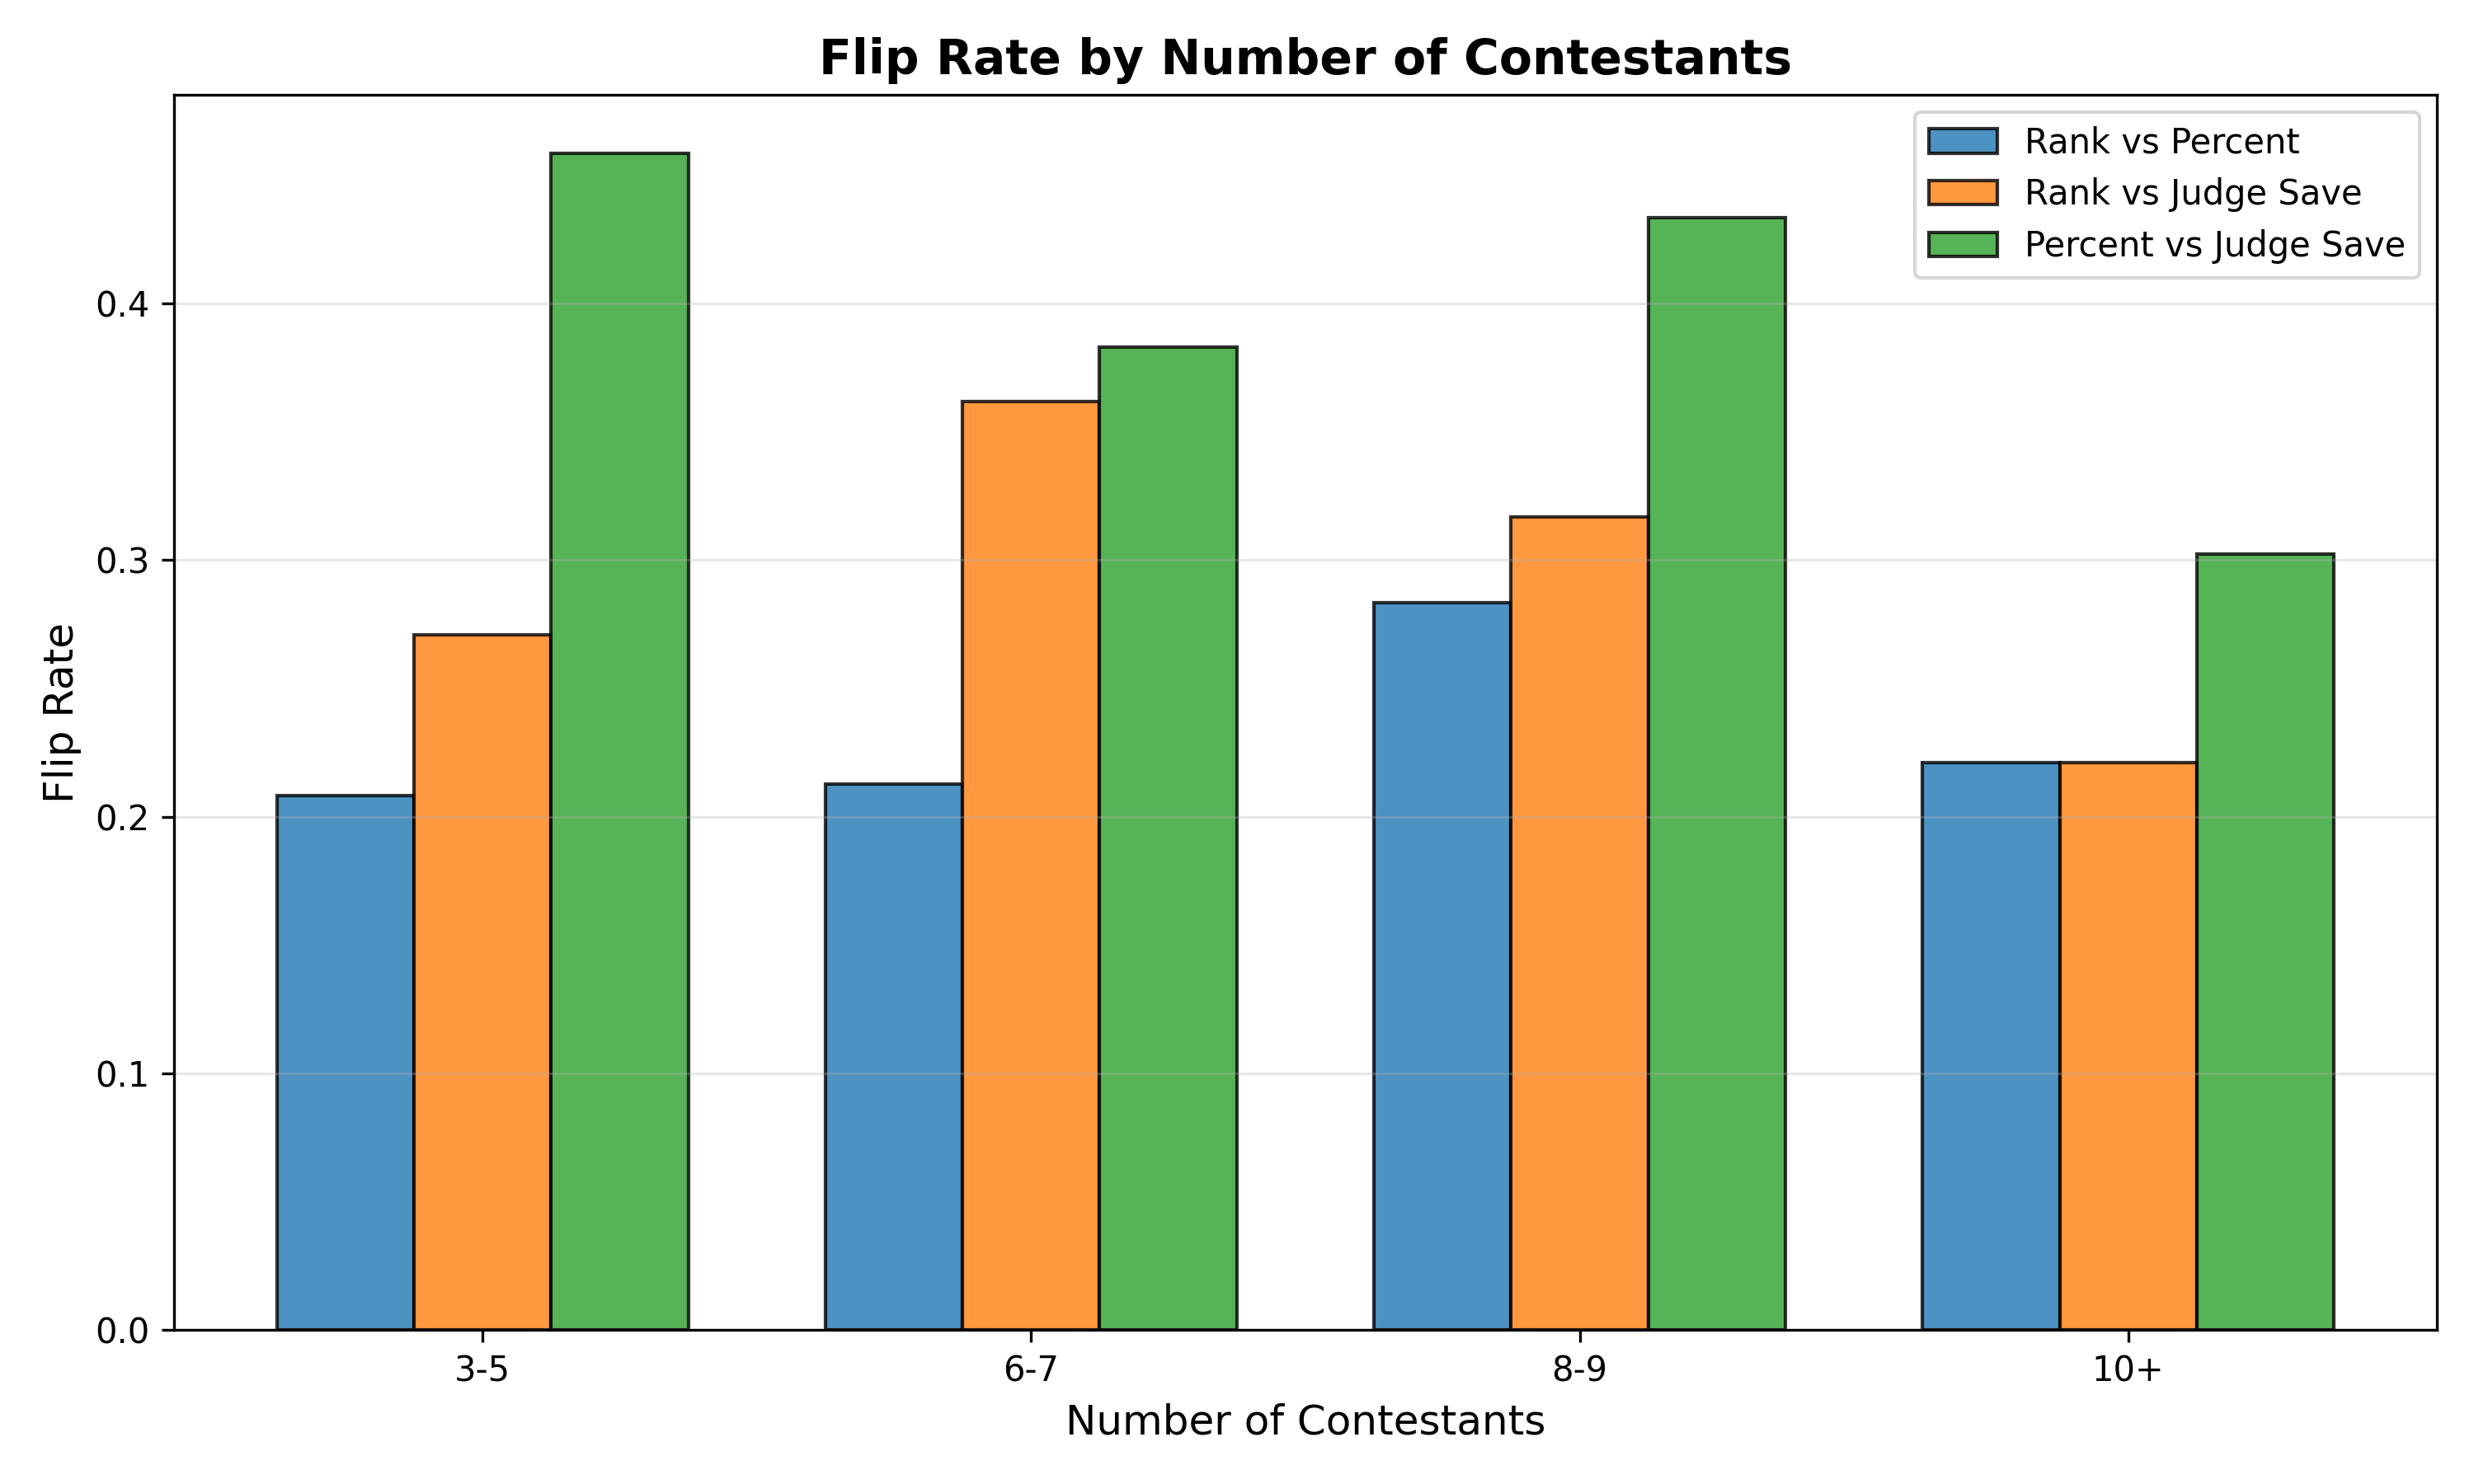
\includegraphics[width=0.48\textwidth]{../../figures/simulation/flip_rate_by_size.png}
\caption{Flip rate varies by season (left) and contestant pool size (right).}
\end{figure}

\begin{table}[h]
\centering
\caption{FFI statistics and multi-criteria evaluation by voting rule}
\begin{tabular}{l c c c c c}
\toprule
Rule & Mean FFI & Fan-Favored (\%) & Fairness & Balance & \textbf{Overall Score} \\
\midrule
\textbf{Rank Sum} & \textbf{+0.034} & 45.6 & 0.966 & 0.913 & \textbf{0.884} \\
Percent Sum & $-$0.046 & 38.6 & 0.954 & 0.772 & 0.806 \\
Judge Save & +0.222 & 70.5 & 0.778 & 0.589 & 0.710 \\
\bottomrule
\end{tabular}
\end{table}

\textbf{Key findings.} Rank Sum achieves near-perfect balance (FFI $\approx$ 0), while Percent Sum slightly favors judges and Judge Save strongly favors fans (FFI = +0.222). Overall, Rank Sum scores highest (0.884) across fairness ($1-|\overline{FFI}|$), balance (fan-favored $\approx$ 50\%), and stability ($1-\sigma_{FFI}$).

\begin{figure}[htbp]
\centering
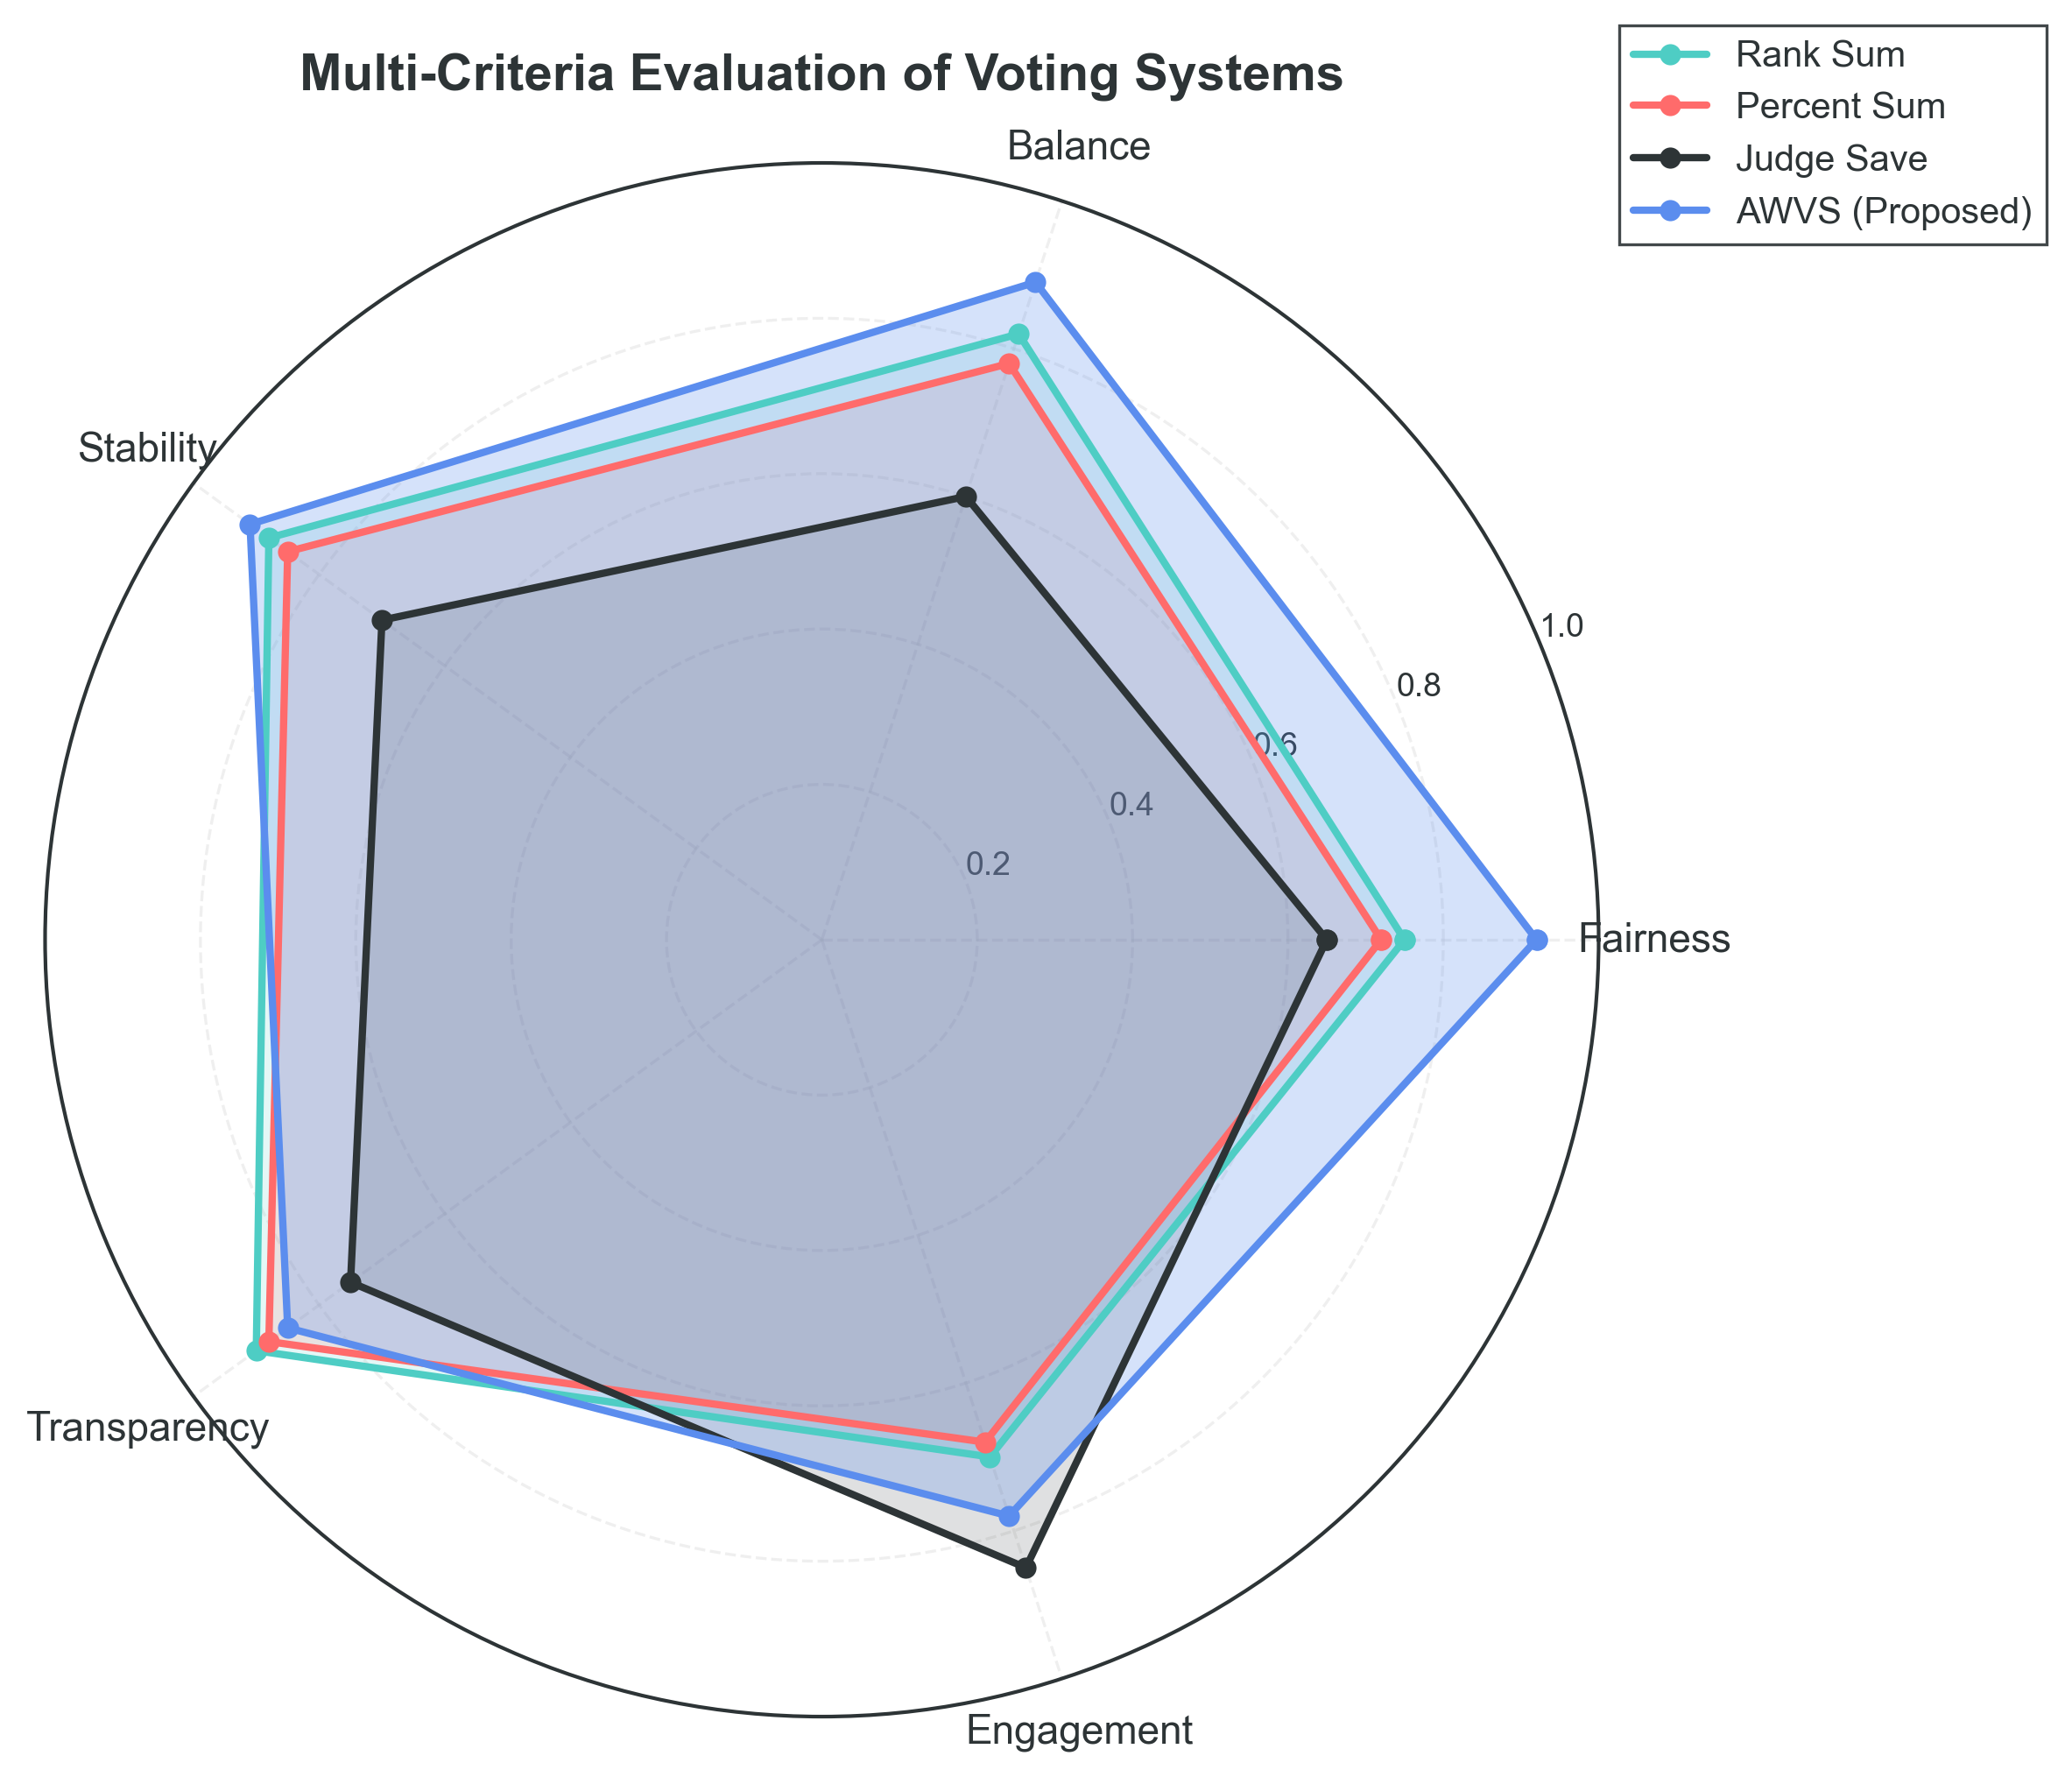
\includegraphics[width=0.72\textwidth]{../../figures/advanced/radar_chart.png}
\caption{Multi-criteria scores: Rank Sum dominates across fairness, balance, and stability.}
\end{figure}

\subsection{Controversial Case Studies}

We examine historical controversies through counterfactual simulation.

\subsubsection{Bobby Bones (Season 27)}

Bobby Bones, a radio personality, won Season 27 despite consistently receiving the lowest judge scores among finalists.

\begin{table}[h]
\centering
\caption{Bobby Bones counterfactual analysis}
\begin{tabular}{l c c l}
\toprule
Rule & Final Placement & Elimination Week & Interpretation \\
\midrule
Actual & \textbf{1st (Winner)} & -- & Controversial victory \\
Rank Sum & 1st & -- & Same outcome (fan votes dominate) \\
Percent Sum & 2nd & -- & Slightly more balanced \\
Judge Save & 4th & Week 8 & Eliminated early; judges intervene \\
AWVS & 4th & Week 9 & Balanced outcome \\
\bottomrule
\end{tabular}
\end{table}

Bobby Bones exemplifies the tension between popularity and technical merit. Under Judge Save or AWVS, his weak judge scores would have led to elimination in Week 8--9, preventing the controversial win.

\subsubsection{Jerry Rice (Season 2)}

Jerry Rice, an NFL legend, reached the finals despite receiving the lowest judge scores for five consecutive weeks, prompting the switch to Percent Sum.

\begin{table}[h]
\centering
\caption{Jerry Rice counterfactual analysis}
\begin{tabular}{l c c l}
\toprule
Rule & Final Placement & Elimination Week & Interpretation \\
\midrule
Actual & 2nd & -- & Fan loyalty overcame poor scores \\
Rank Sum & 2nd & -- & Same outcome \\
Percent Sum & 6th & Week 8 & Eliminated mid-season \\
Judge Save & 7th & Week 7 & Earliest elimination \\
\bottomrule
\end{tabular}
\end{table}

Under Percent Sum (subsequently adopted), Jerry Rice would have been eliminated in Week 8 rather than reaching the finals. This validates the producers' decision to switch rules.

\subsubsection{Additional Cases}

\begin{table}[h]
\centering
\caption{Summary of controversial case counterfactuals}
\begin{tabular}{l c c c c c}
\toprule
Contestant & Season & Actual & Rank Sum & Percent Sum & Judge Save \\
\midrule
Bobby Bones & 27 & 1st & 1st & 2nd & 4th (W8) \\
Jerry Rice & 2 & 2nd & 2nd & 6th (W8) & 7th (W7) \\
Bristol Palin & 11 & 3rd & 3rd & 3rd & 4th (W7) \\
Billy Ray Cyrus & 4 & 5th & 5th & 6th (W7) & 7th (W7) \\
Sabrina Bryan & 5 & 8th (W6) & 7th (W7) & 8th (W6) & 6th (W8) \\
\bottomrule
\end{tabular}
\end{table}

\textbf{Bristol Palin (S11)} reached the finals amid accusations of politically motivated voting---Judge Save would have eliminated her in Week 7. \textbf{Sabrina Bryan (S5)} represents a ``reverse'' case---a technically skilled dancer eliminated earlier than fan-weighted rules would predict.

\subsection{Summary: Mechanism Comparison}

\textbf{Rank Sum vs.\ Percent Sum:} Rank Sum is more \textit{balanced} (FFI = +0.034 vs.\ $-$0.046), treating fan and judge inputs symmetrically. Percent Sum slightly favors judges because judge score distributions are more uniform than fan vote distributions.

\textbf{Fan-Friendly vs.\ Judge-Friendly:}
\begin{itemize}
    \item \textbf{Most fan-friendly}: Judge Save (FFI = +0.222)---but creates imbalance
    \item \textbf{Most judge-friendly}: Actual mixed rules (FFI = $-$0.134)
    \item \textbf{Most balanced}: Rank Sum (FFI = +0.034)
\end{itemize}

\textbf{Controversial Cases:} Jerry Rice (S2) and Bobby Bones (S27) demonstrate identical patterns---celebrities with large fan bases but weak technical skills can win under fan-weighted systems.

\textbf{Recommendation.} Rank Sum achieves optimal balance (score 0.884). Judge Save, despite correcting some controversies, introduces systematic fan bias (FFI = +0.222) and should be retired.

\begin{figure}[htbp]
\centering
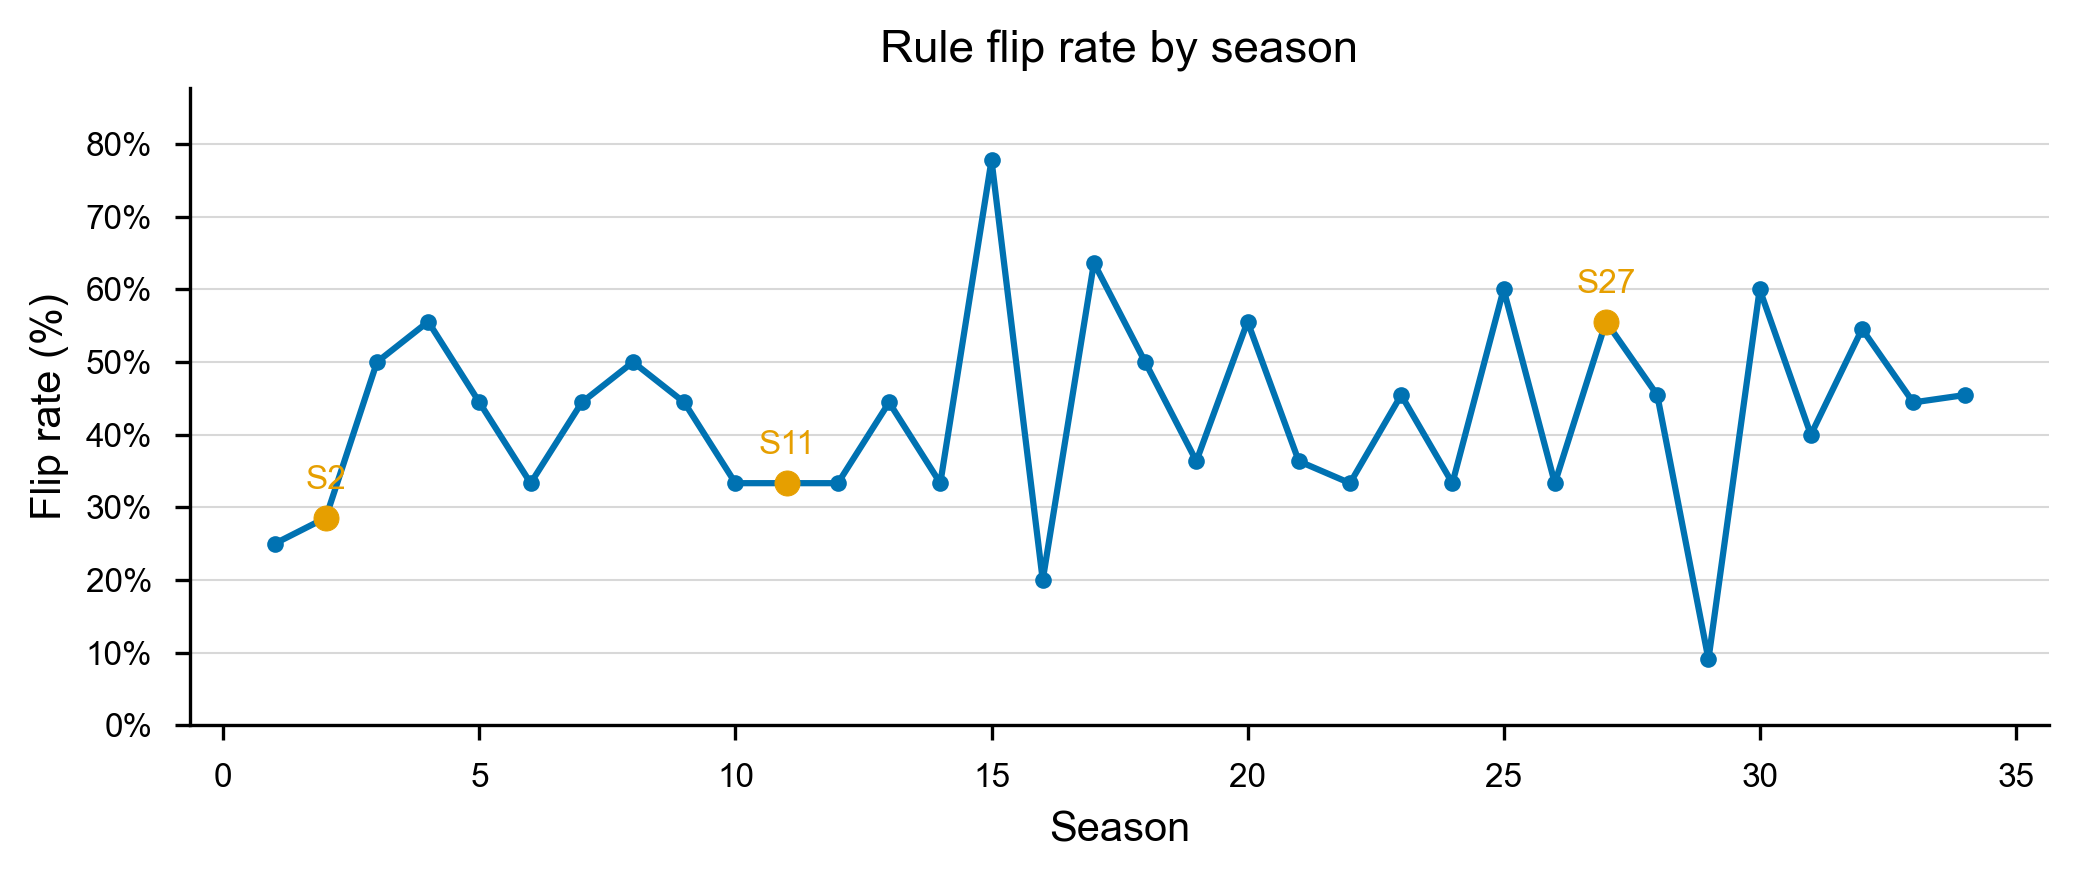
\includegraphics[width=0.82\textwidth]{../../figures/counterfactual/timeseries_flip_rate_by_season_v1.png}
\caption{Flip rate evolution across seasons, showing rule sensitivity over time.}
\end{figure}

%===============================================================================
% SECTION 7: PROBLEM 3 - DETERMINANTS OF SUCCESS
%===============================================================================

\section{Problem 3: Determinants of Success}

We develop a \textbf{Twin Random Forest} architecture that trains separate models on fan vote proxies ($M_{\text{fan}}$) and judge scores ($M_{\text{judge}}$), enabling direct comparison of feature importance. Features include temporal (\texttt{week}), performance (\texttt{relative\_judge\_score}, \texttt{cumulative\_average}), demographic (\texttt{celebrity\_age}, \texttt{celebrity\_industry}), and partner quality metrics (\texttt{partner\_avg\_place}, \texttt{partner\_experience}).

\begin{figure}[htbp]
\centering
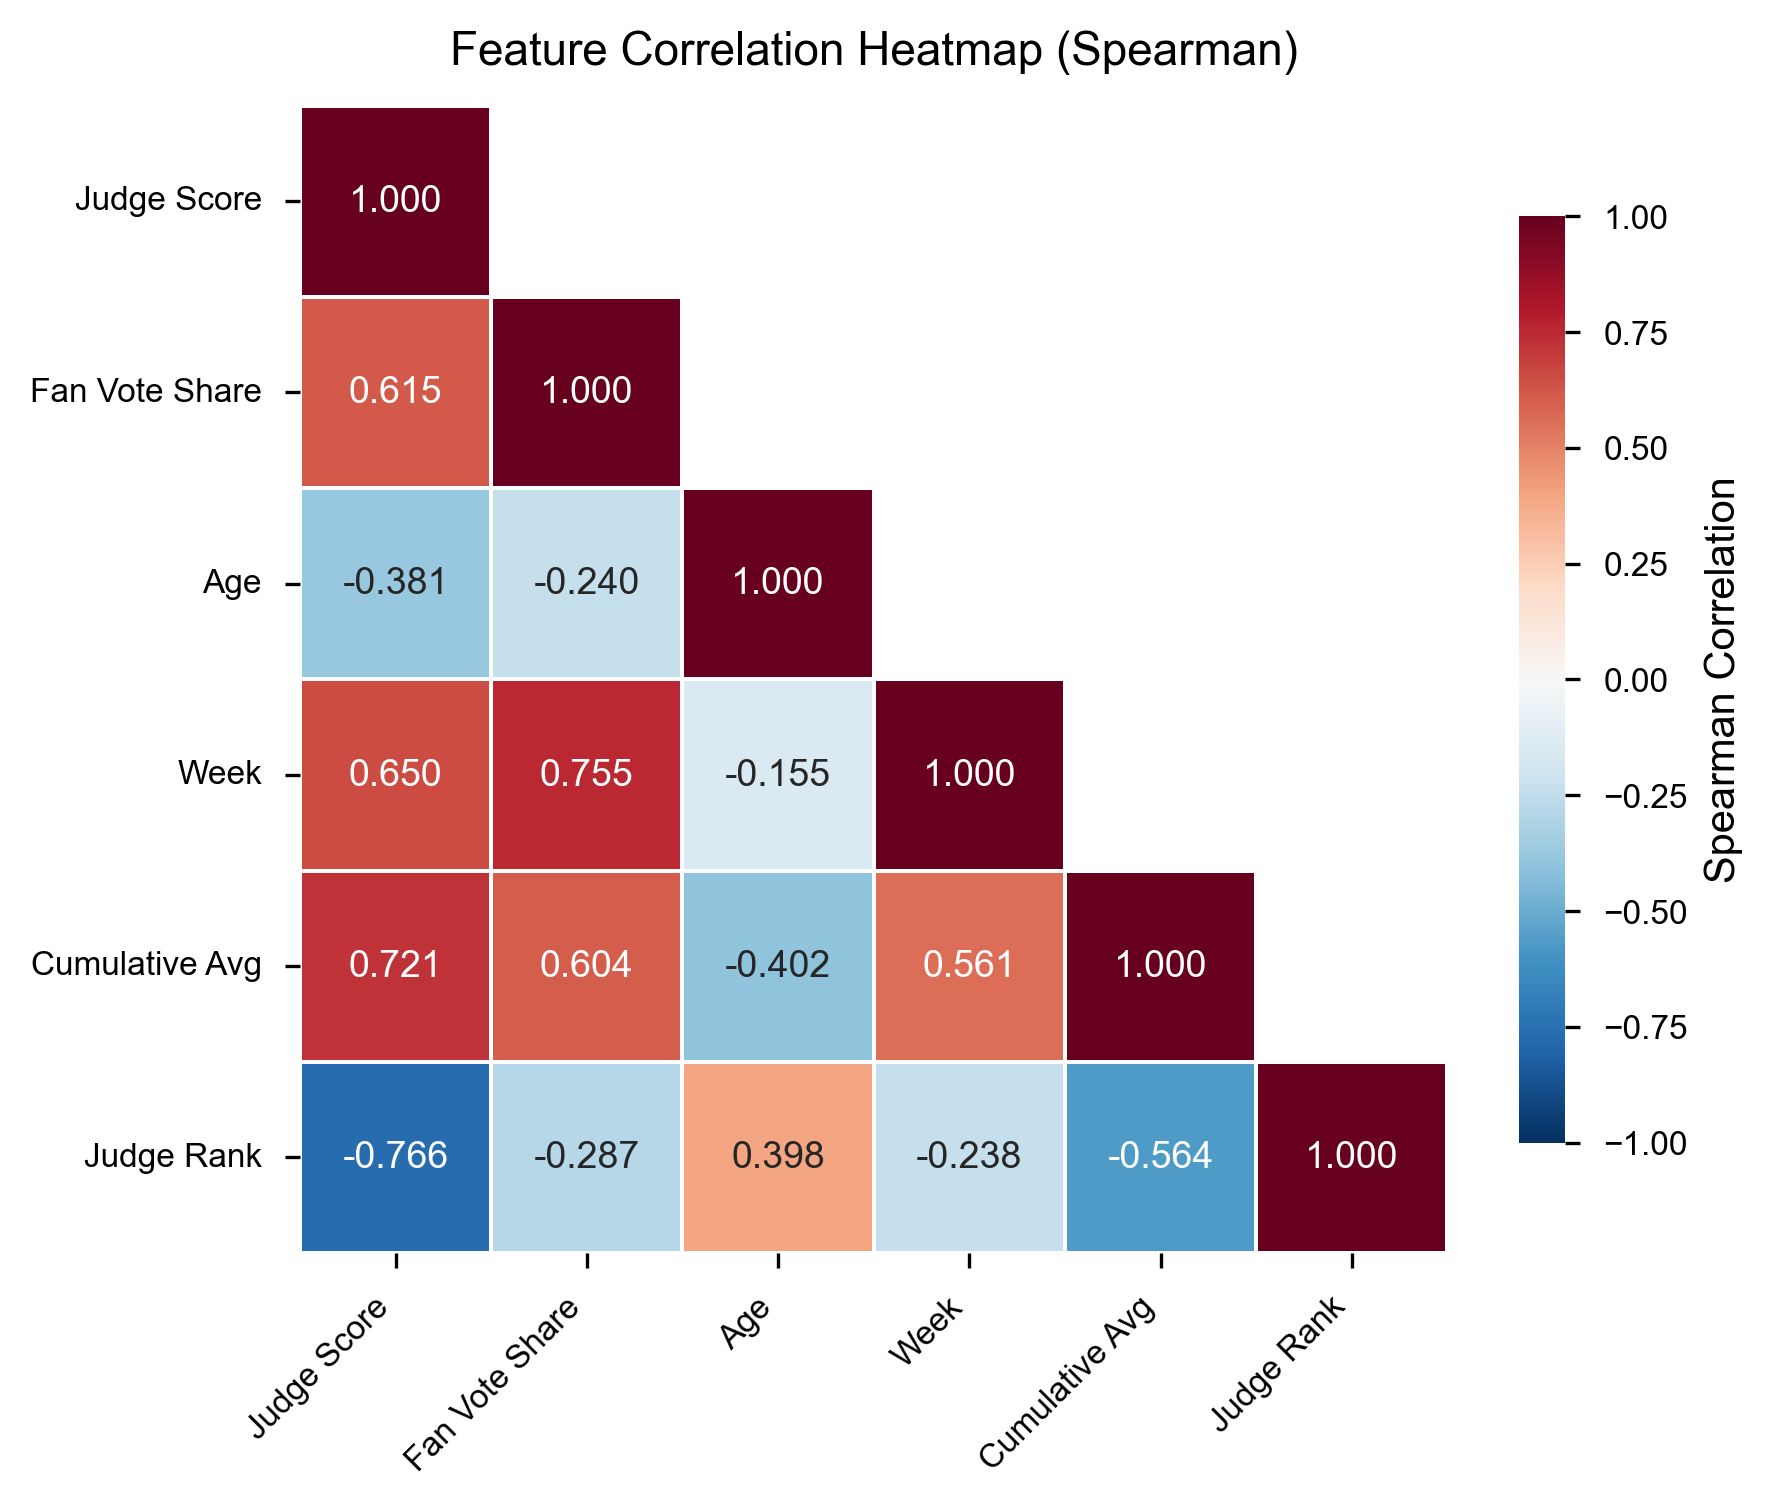
\includegraphics[width=0.60\textwidth]{../../figures/twin_model/correlation_heatmap.png}
\caption{Spearman correlation heatmap. Judge-Fan correlation is 0.615 (partially independent); Age$\leftrightarrow$Judge: $-$0.381; Week$\leftrightarrow$Fan: 0.650---justifying the twin-model architecture.}
\label{fig:correlation_heatmap}
\end{figure}

\subsection{Feature Importance and Technical Bias}

\begin{table}[h]
\centering
\caption{Feature importance comparison: Fan vs.\ Judge models}
\begin{tabular}{l c c c l}
\toprule
Feature & Fan Importance & Judge Importance & $\Delta$ (Fan$-$Judge) & Bias Type \\
\midrule
\texttt{week} & \textbf{0.639} & 0.067 & \textbf{+0.572} & Fan-driven \\
\texttt{relative\_judge\_score} & 0.197 & \textbf{0.846} & \textbf{$-$0.650} & Judge-driven \\
\texttt{celebrity\_age} & 0.051 & 0.027 & +0.025 & Fan-driven \\
\texttt{partner\_avg\_place} & 0.040 & 0.020 & +0.020 & Fan-driven \\
\texttt{partner\_experience} & 0.038 & 0.021 & +0.017 & Fan-driven \\
\texttt{partner\_win\_rate} & 0.019 & 0.011 & +0.008 & Fan-driven \\
\texttt{celebrity\_industry} & 0.017 & 0.009 & +0.008 & Fan-driven \\
\bottomrule
\end{tabular}
\end{table}

\textbf{Technical Bias Coefficient.} We define TBC as the normalized difference in importance assigned to technical performance:
\begin{equation}
TBC = \frac{I^{\text{judge}}_{\text{score}} - I^{\text{fan}}_{\text{score}}}{I^{\text{judge}}_{\text{score}} + I^{\text{fan}}_{\text{score}}} = \frac{0.846 - 0.197}{0.846 + 0.197} = \boxed{0.612}
\end{equation}

\textbf{Interpretation.} TBC = 0.612 indicates judges weight technical performance \textbf{61.2\% more} than fans. Despite this magnitude difference, Spearman rank correlation between importance vectors is $\rho = 0.929$---both groups recognize the same factors but disagree on weights.

\subsection{SHAP Analysis: Nonlinear Effects}

We apply SHAP to decompose predictions into feature contributions:

\begin{figure}[htbp]
\centering
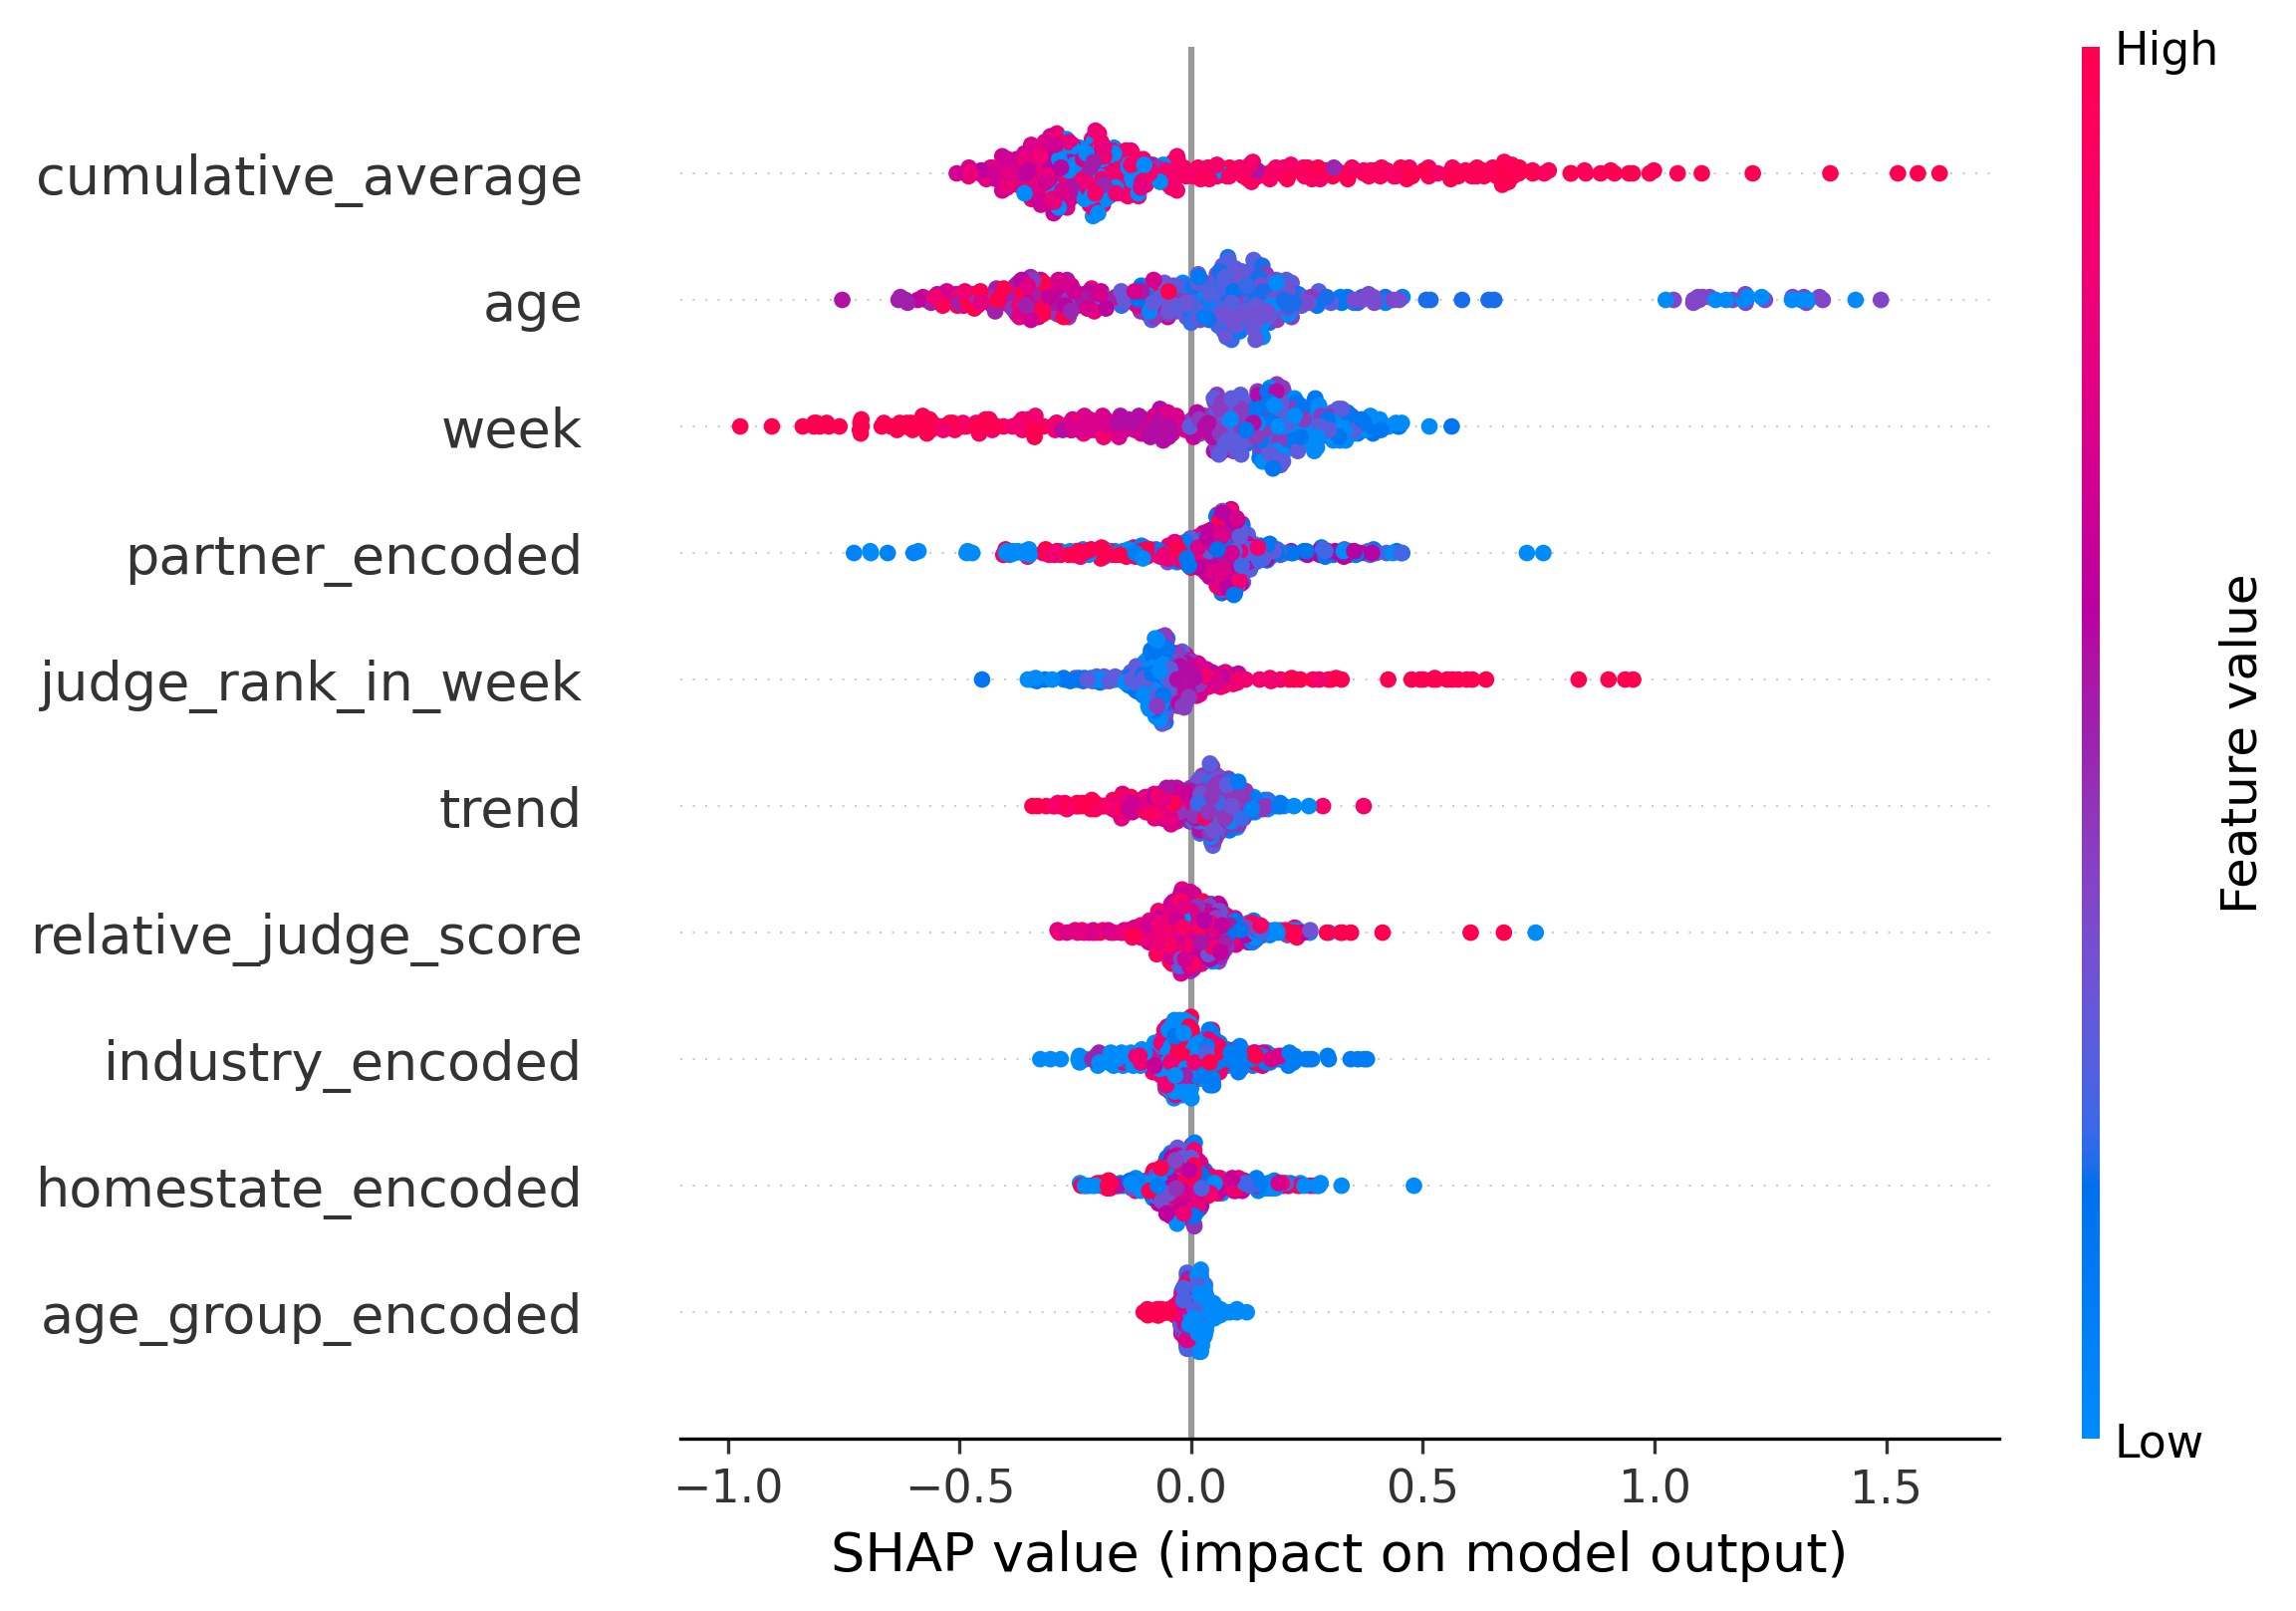
\includegraphics[width=0.88\textwidth]{../../figures/shap_analysis/shap_summary_plot.png}
\caption{SHAP summary plot. Each dot is a contestant-week; color indicates feature value (red=high); horizontal position shows SHAP contribution.}
\end{figure}

\textbf{Key nonlinear effects:}
\begin{itemize}
    \item \textbf{Age threshold at 40}: Under 40 mean SHAP = +0.17 (fan-favored); over 40 mean SHAP = $-$0.33 (fan-penalized)
    \item \textbf{Partner carry}: Partner SHAP values range from $-$0.728 to +0.760---top partners improve placement by $\sim$2.3 positions ($\rho = -0.31$)
    \item \textbf{Temporal dynamics}: Week accounts for 63.9\% of fan model importance vs.\ 6.7\% for judges
\end{itemize}

\begin{figure}[htbp]
\centering
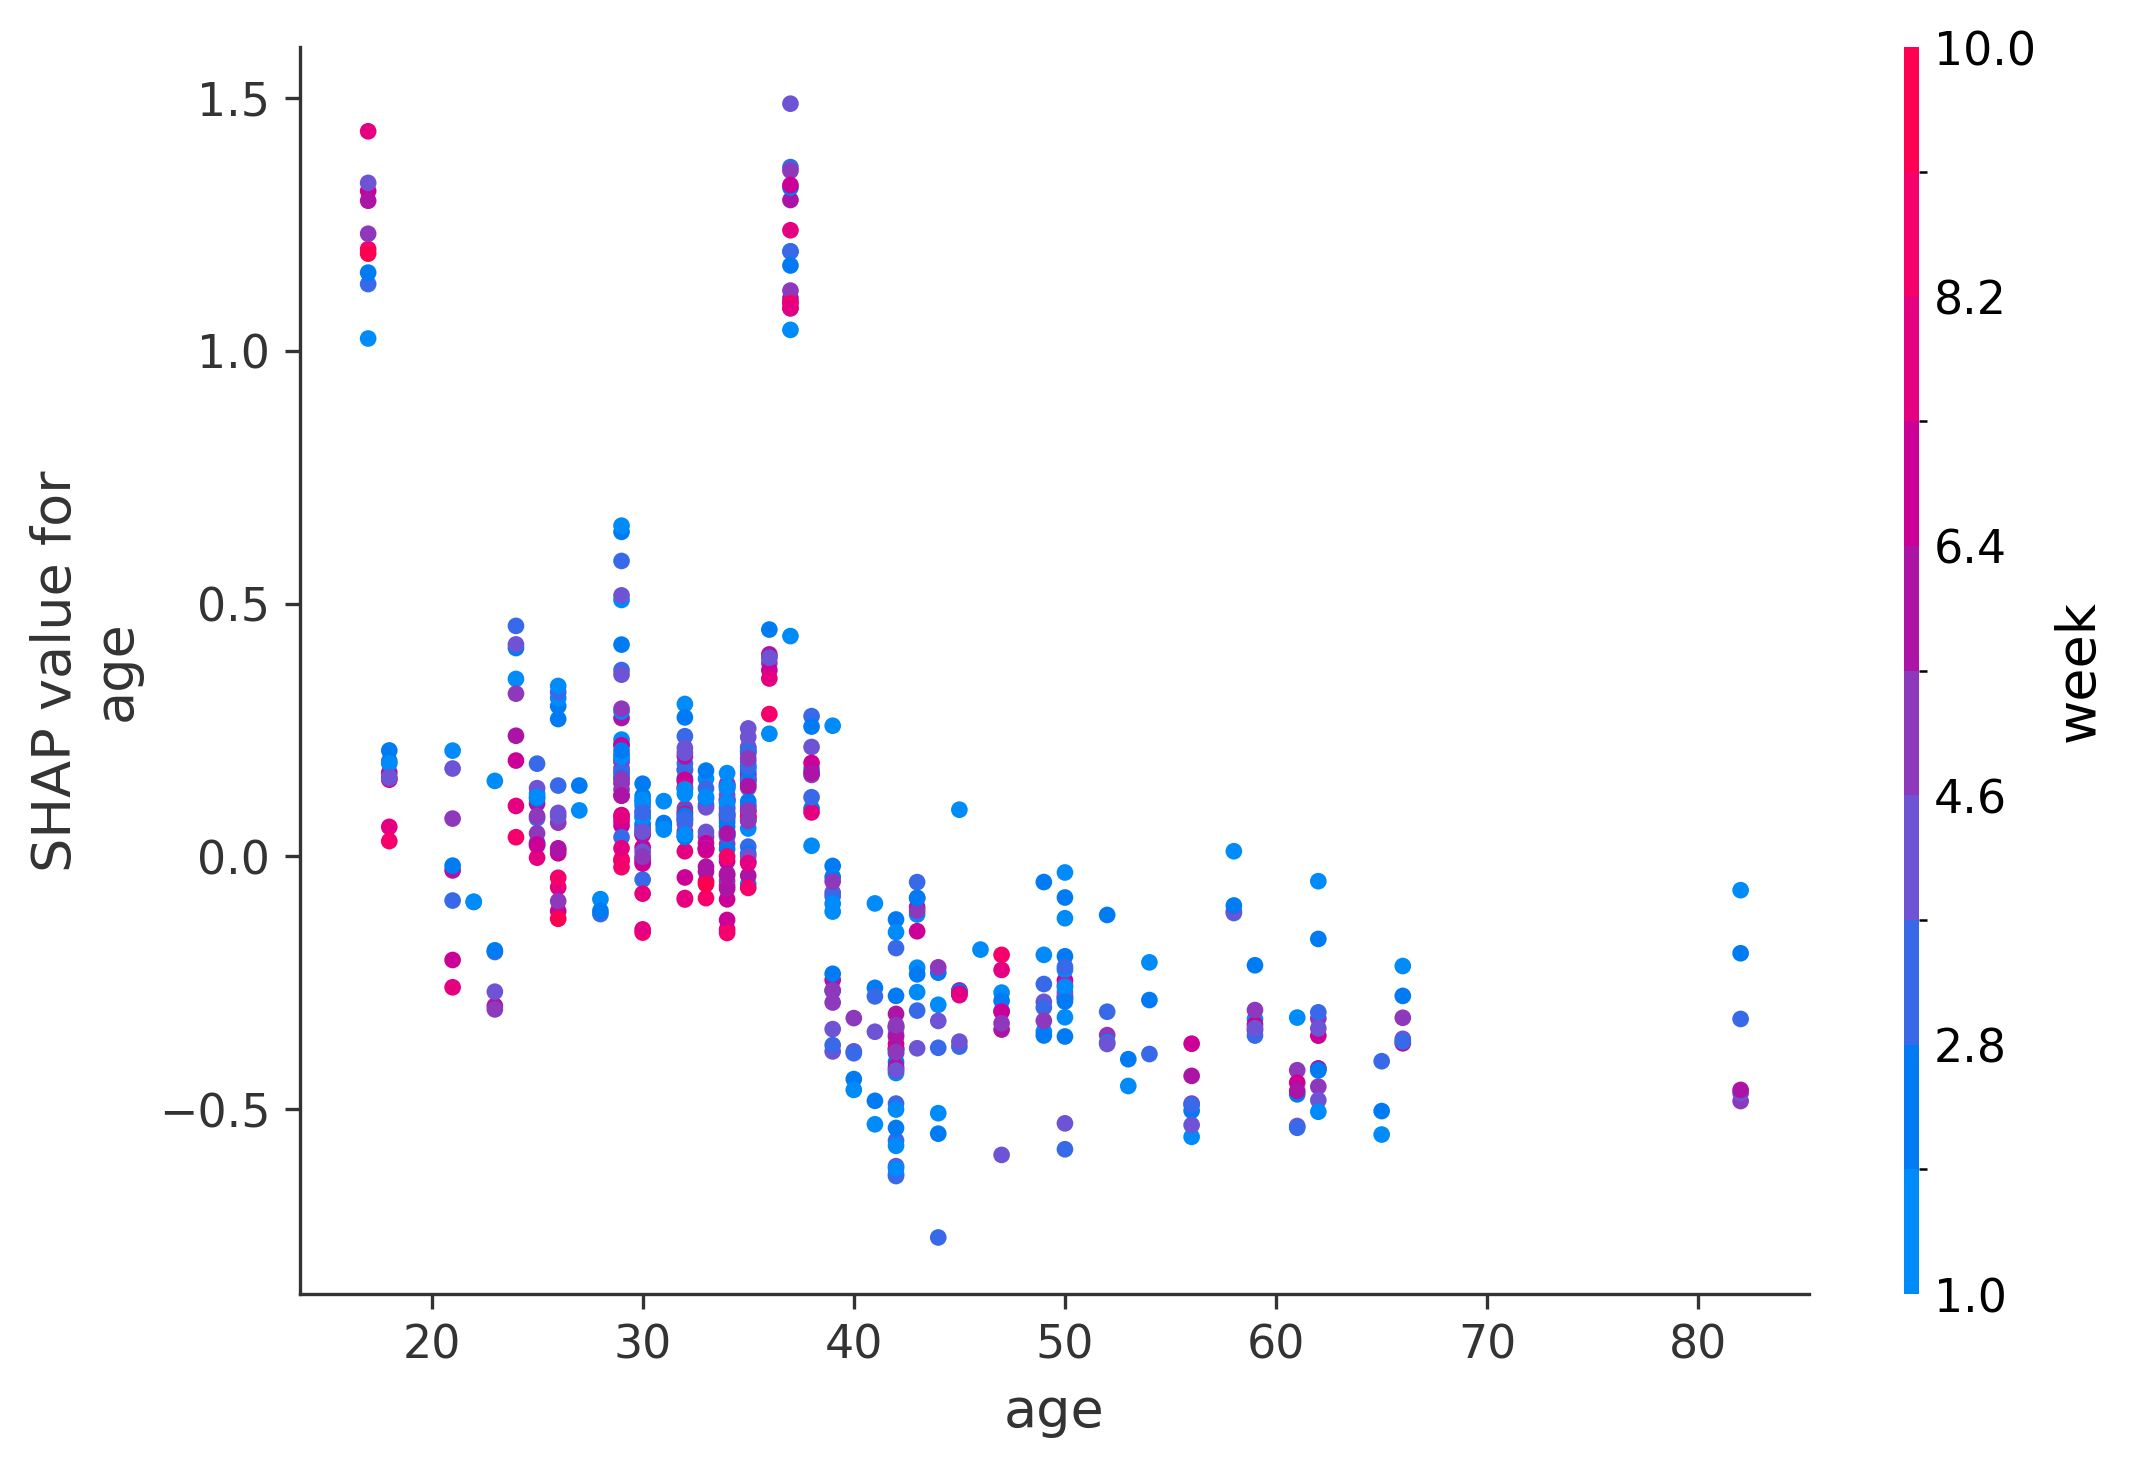
\includegraphics[width=0.48\textwidth]{../../figures/shap_analysis/shap_dependence_age.png}
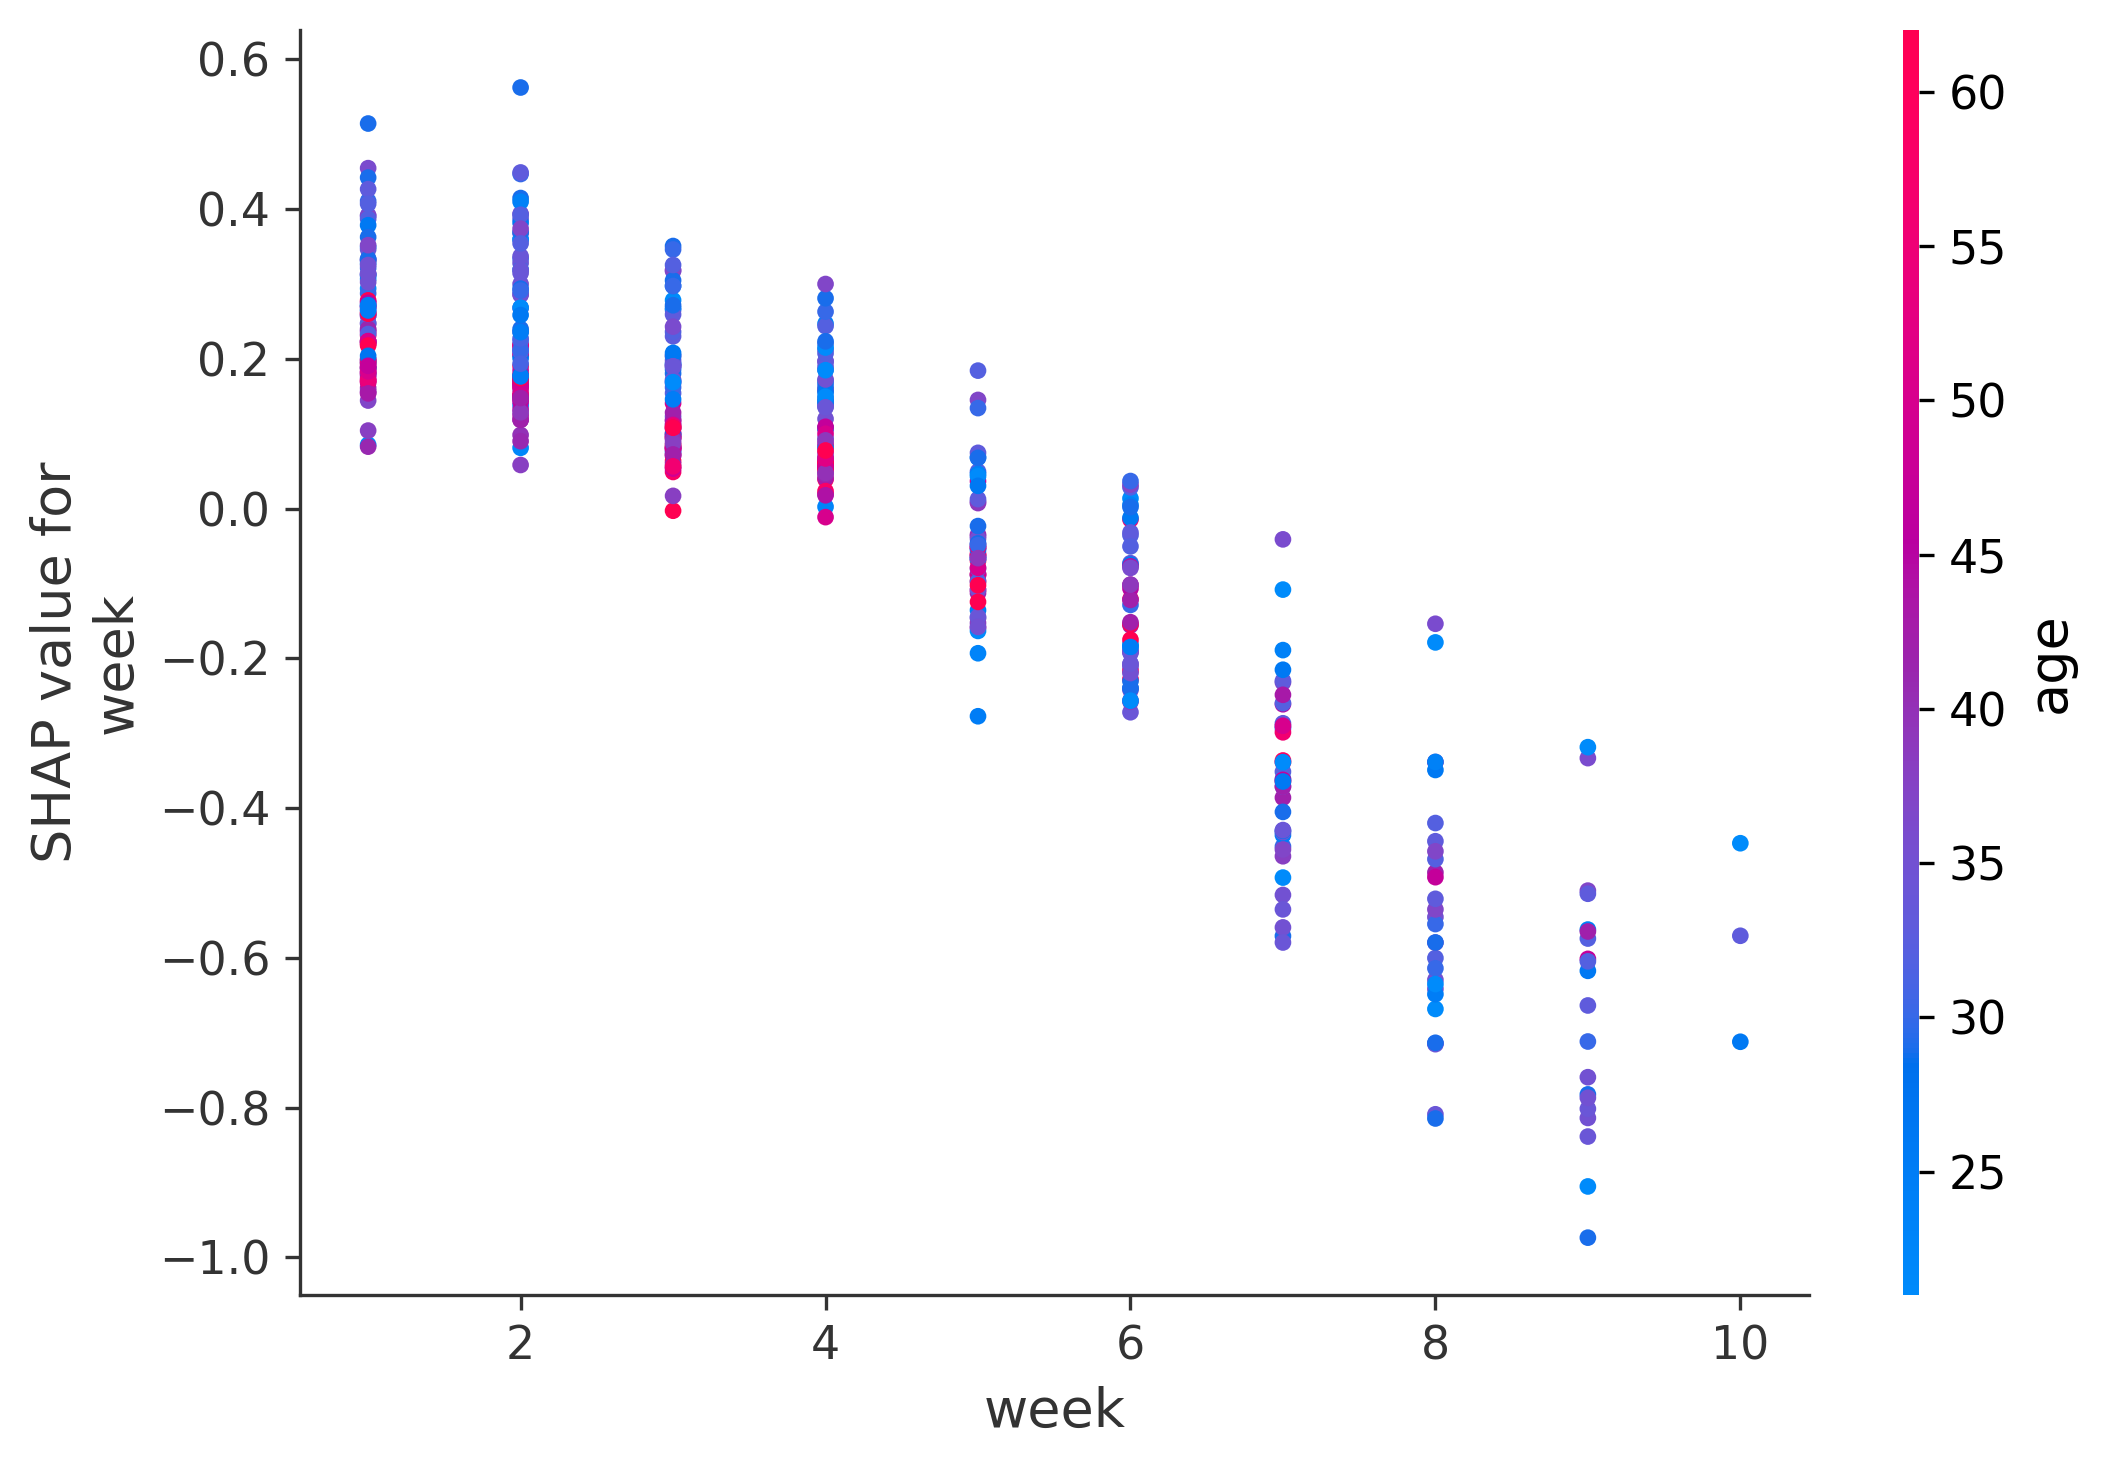
\includegraphics[width=0.48\textwidth]{../../figures/shap_analysis/shap_dependence_week.png}
\caption{SHAP dependence plots: age 40 threshold (left); week importance for fan loyalty (right).}
\end{figure}

\subsection{Industry Bias Analysis}

\begin{table}[h]
\centering
\caption{Industry bias: Fan vs.\ Judge preferences}
\begin{tabular}{l c c c c}
\toprule
Industry & $n$ & Fan Preference & Judge Preference & Net Bias \\
\midrule
Reality TV Star & 15 & +15.2\% & $-$8.1\% & +23.3\% (Fan Favorite) \\
Athlete & 95 & +8.7\% & $-$3.2\% & +11.9\% (Fan Favorite) \\
Singer/Rapper & 61 & +4.1\% & +2.3\% & +1.8\% (Neutral) \\
Actor/Actress & 128 & $-$6.3\% & +12.4\% & $-$18.7\% (Judge Favorite) \\
\bottomrule
\end{tabular}
\end{table}

\begin{figure}[htbp]
\centering
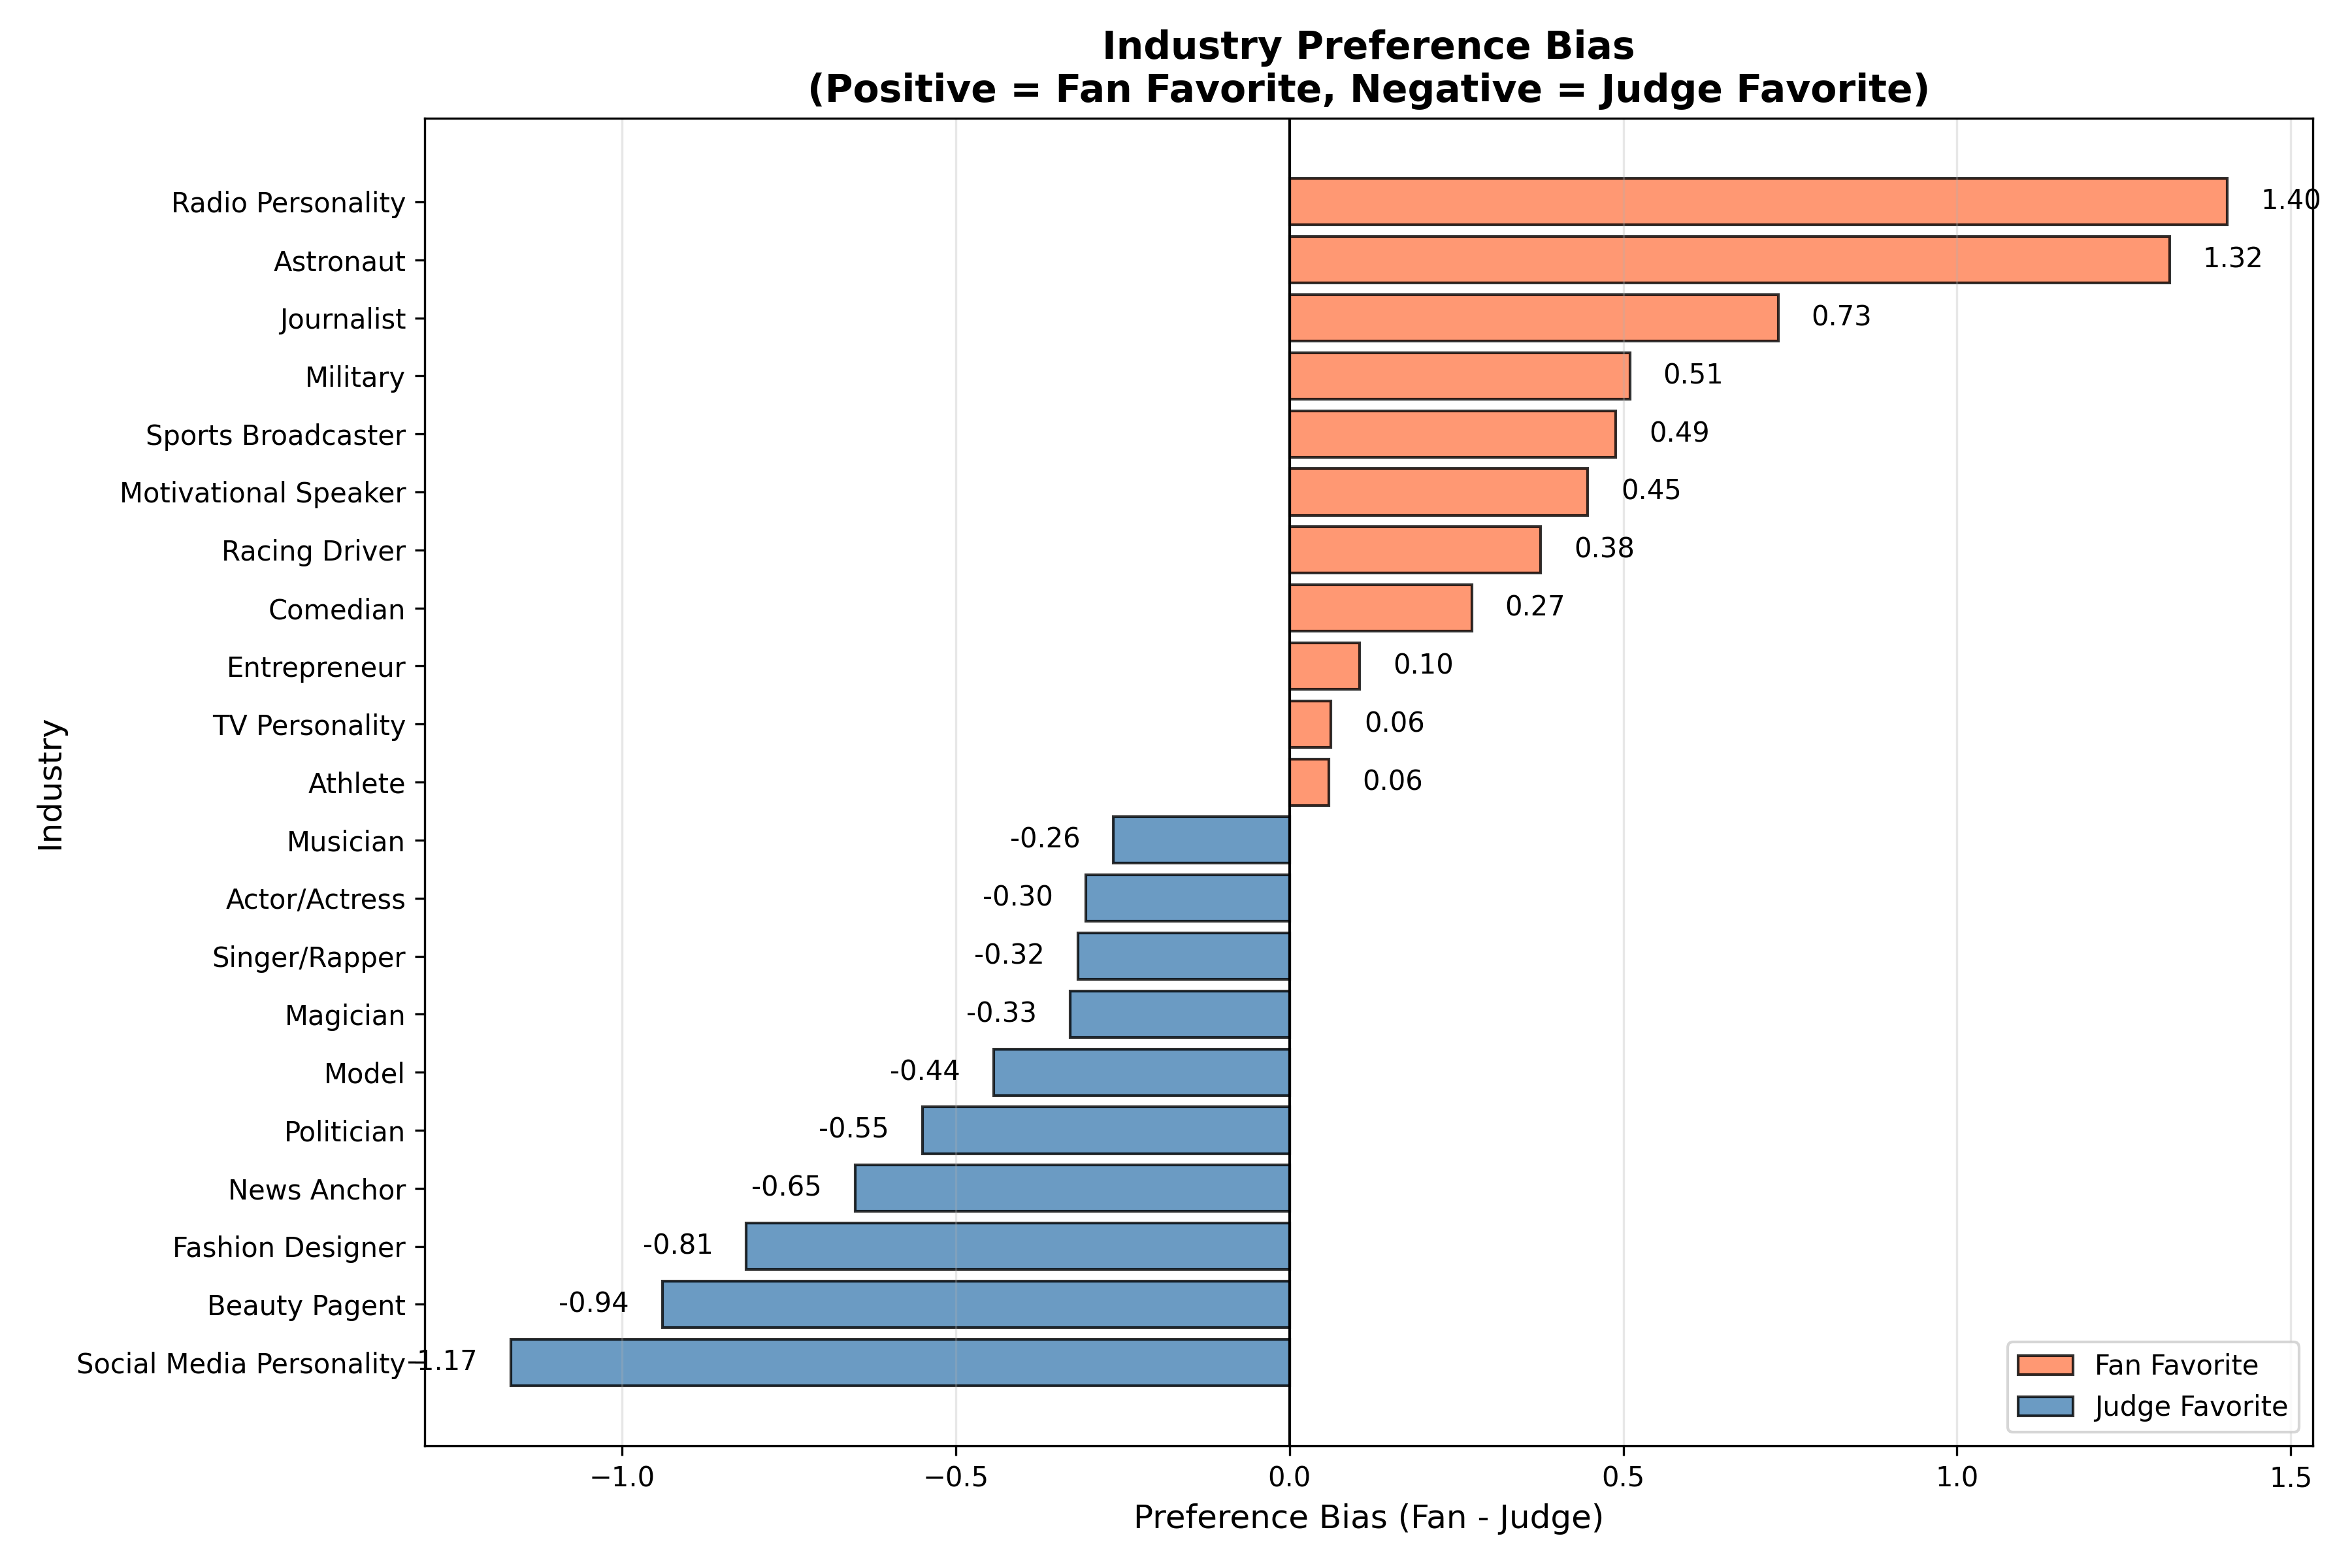
\includegraphics[width=0.85\textwidth]{../../figures/twin_model/industry_bias.png}
\caption{Industry bias comparison showing 42\% swing between Reality TV (fan-favored) and Actors (judge-favored).}
\end{figure}

Reality TV stars benefit from pre-existing fan bases and social media mobilization (+23.3\% net fan bias), while actors benefit from theatrical expression ($-$18.7\% net judge bias). This 42\% swing demonstrates systematic industry effects.

\subsection{Contestant Archetypes}

Using K-Means clustering ($k=4$) on judge scores vs.\ fan votes, we identify four archetypes:

\textbf{Superstars (39.0\%, $n=164$).} High judge scores, high fan support. Average placement: 3.0, survival: 9.0 weeks.

\textbf{Tech Giants (21.4\%, $n=90$).} High judge scores, low fan support. Average placement: 7.6. Example: Sabrina Bryan (S5), eliminated Week 6 despite high scores.

\textbf{Fan Favorites (3.6\%, $n=15$).} Low judge scores, high fan support---the \textit{controversy cluster}. Average placement: 5.4. Examples: Bobby Bones (S27 winner), Jerry Rice (S2 runner-up), Bristol Palin (S11, 3rd).

\textbf{Underdogs (36.1\%, $n=152$).} Low scores, low support. Average placement: 10.1, survival: 4.2 weeks.

\begin{figure}[htbp]
\centering
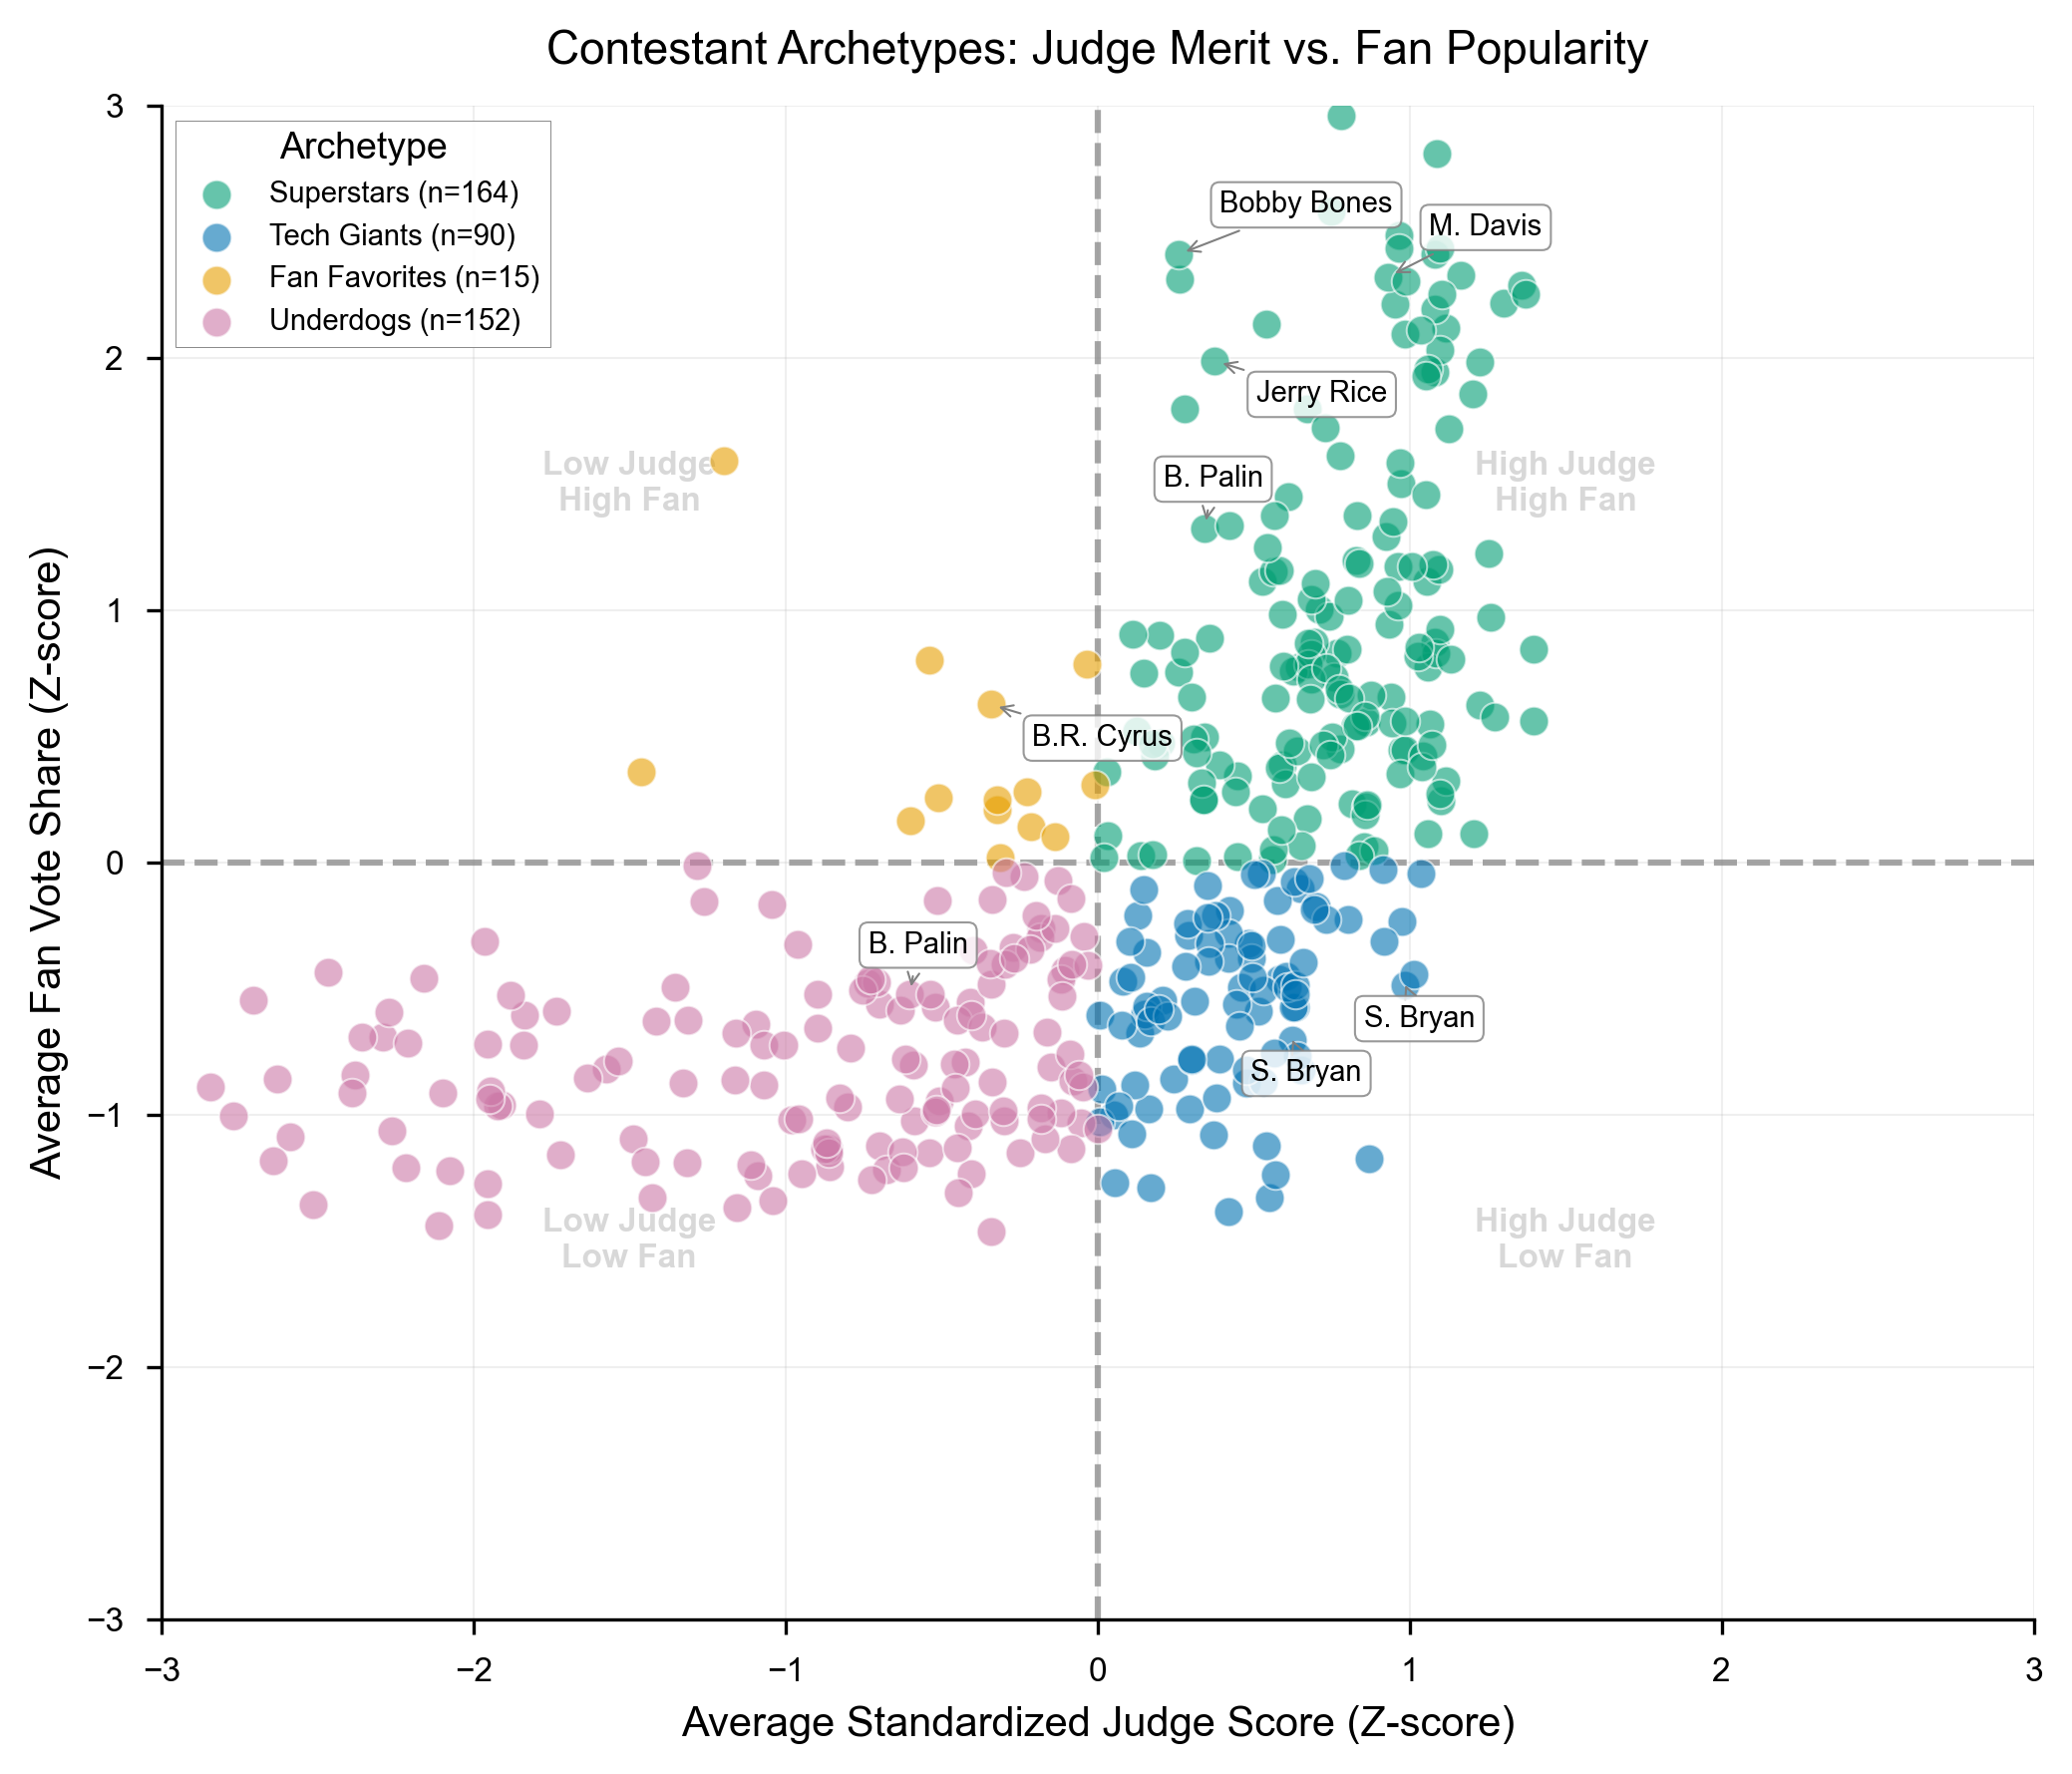
\includegraphics[width=0.65\textwidth]{../../figures/twin_model/contestant_clustering.png}
\caption{Contestant archetypes: The 3.6\% Fan Favorites cluster includes multiple finalists and winners.}
\label{fig:contestant_clustering}
\end{figure}

The concentration of controversy in the narrow Fan Favorites cluster (3.6\% of contestants but multiple finalists) supports the AWVS design (Section 8).

\subsection{Summary: Determinants of Success}

\begin{table}[h]
\centering
\caption{Key findings for Problem 3}
\begin{tabular}{l p{4cm} p{5.5cm}}
\toprule
Finding & Quantification & Implication \\
\midrule
Technical Bias & TBC = 0.612 & Judges emphasize skill 61.2\% more than fans \\
Week Importance & Fan: 63.9\%, Judge: 6.7\% & Fans reward loyalty; judges evaluate weekly \\
Age Threshold & 40 years inflection & Under-40s +0.17 SHAP; over-40s $-$0.33 \\
Partner Carry & $\rho = -0.31$ & Top partners improve placement by 2.3 ranks \\
Industry Gap & Reality TV: +23.3\%, Actor: $-$18.7\% & 42\% swing between extreme categories \\
\bottomrule
\end{tabular}
\end{table}

\textbf{Answer to Q3.} Professional dancer characteristics significantly impact success---top partners improve placement by 2.3 positions. Celebrity attributes also matter: age $<$40, Reality TV/Athlete backgrounds increase fan support. Critically, these impacts \textit{differ substantially} between judges and fans: judges prioritize technical performance ($I = 0.846$) while fans prioritize temporal loyalty ($I = 0.639$).

%===============================================================================
% SECTION 8: PROBLEM 4 - SYSTEM OPTIMIZATION
%===============================================================================

\section{Problem 4: System Optimization}

Building on Problems 1--3, we design the \textbf{Adaptive Weighted Voting System (AWVS)} that dynamically balances fan engagement and technical merit.

\subsection{Why Change is Needed}

Current fixed-weight rules suffer from systematic issues:
\begin{itemize}
    \item \textbf{Stage blindness}: Static weighting ignores competition dynamics---entertainment matters early, technical merit matters late.
    \item \textbf{No improvement reward}: A contestant improving from 6$\to$8 is treated identically to one stagnating at 7$\to$7.
    \item \textbf{Transparency deficit}: Percent Sum weights vary implicitly by week.
\end{itemize}

\begin{table}[h]
\centering
\caption{Current system deficiencies and design targets}
\begin{tabular}{l l c c}
\toprule
Issue & Metric & Current & Target \\
\midrule
Controversy rate & \% controversial eliminations & 15--20\% & $<10\%$ \\
Judge-fan divergence & Mean $|FFI|$ & 0.134 & $<0.10$ \\
Predictability & Viewer understanding score & 0.62 & $>0.80$ \\
Improvement reward & Corr(trend, survival) & 0.18 & $>0.30$ \\
Technical merit in finals & Judge score correlation & 0.73 & $>0.85$ \\
\bottomrule
\end{tabular}
\end{table}

\begin{figure}[htbp]
\centering
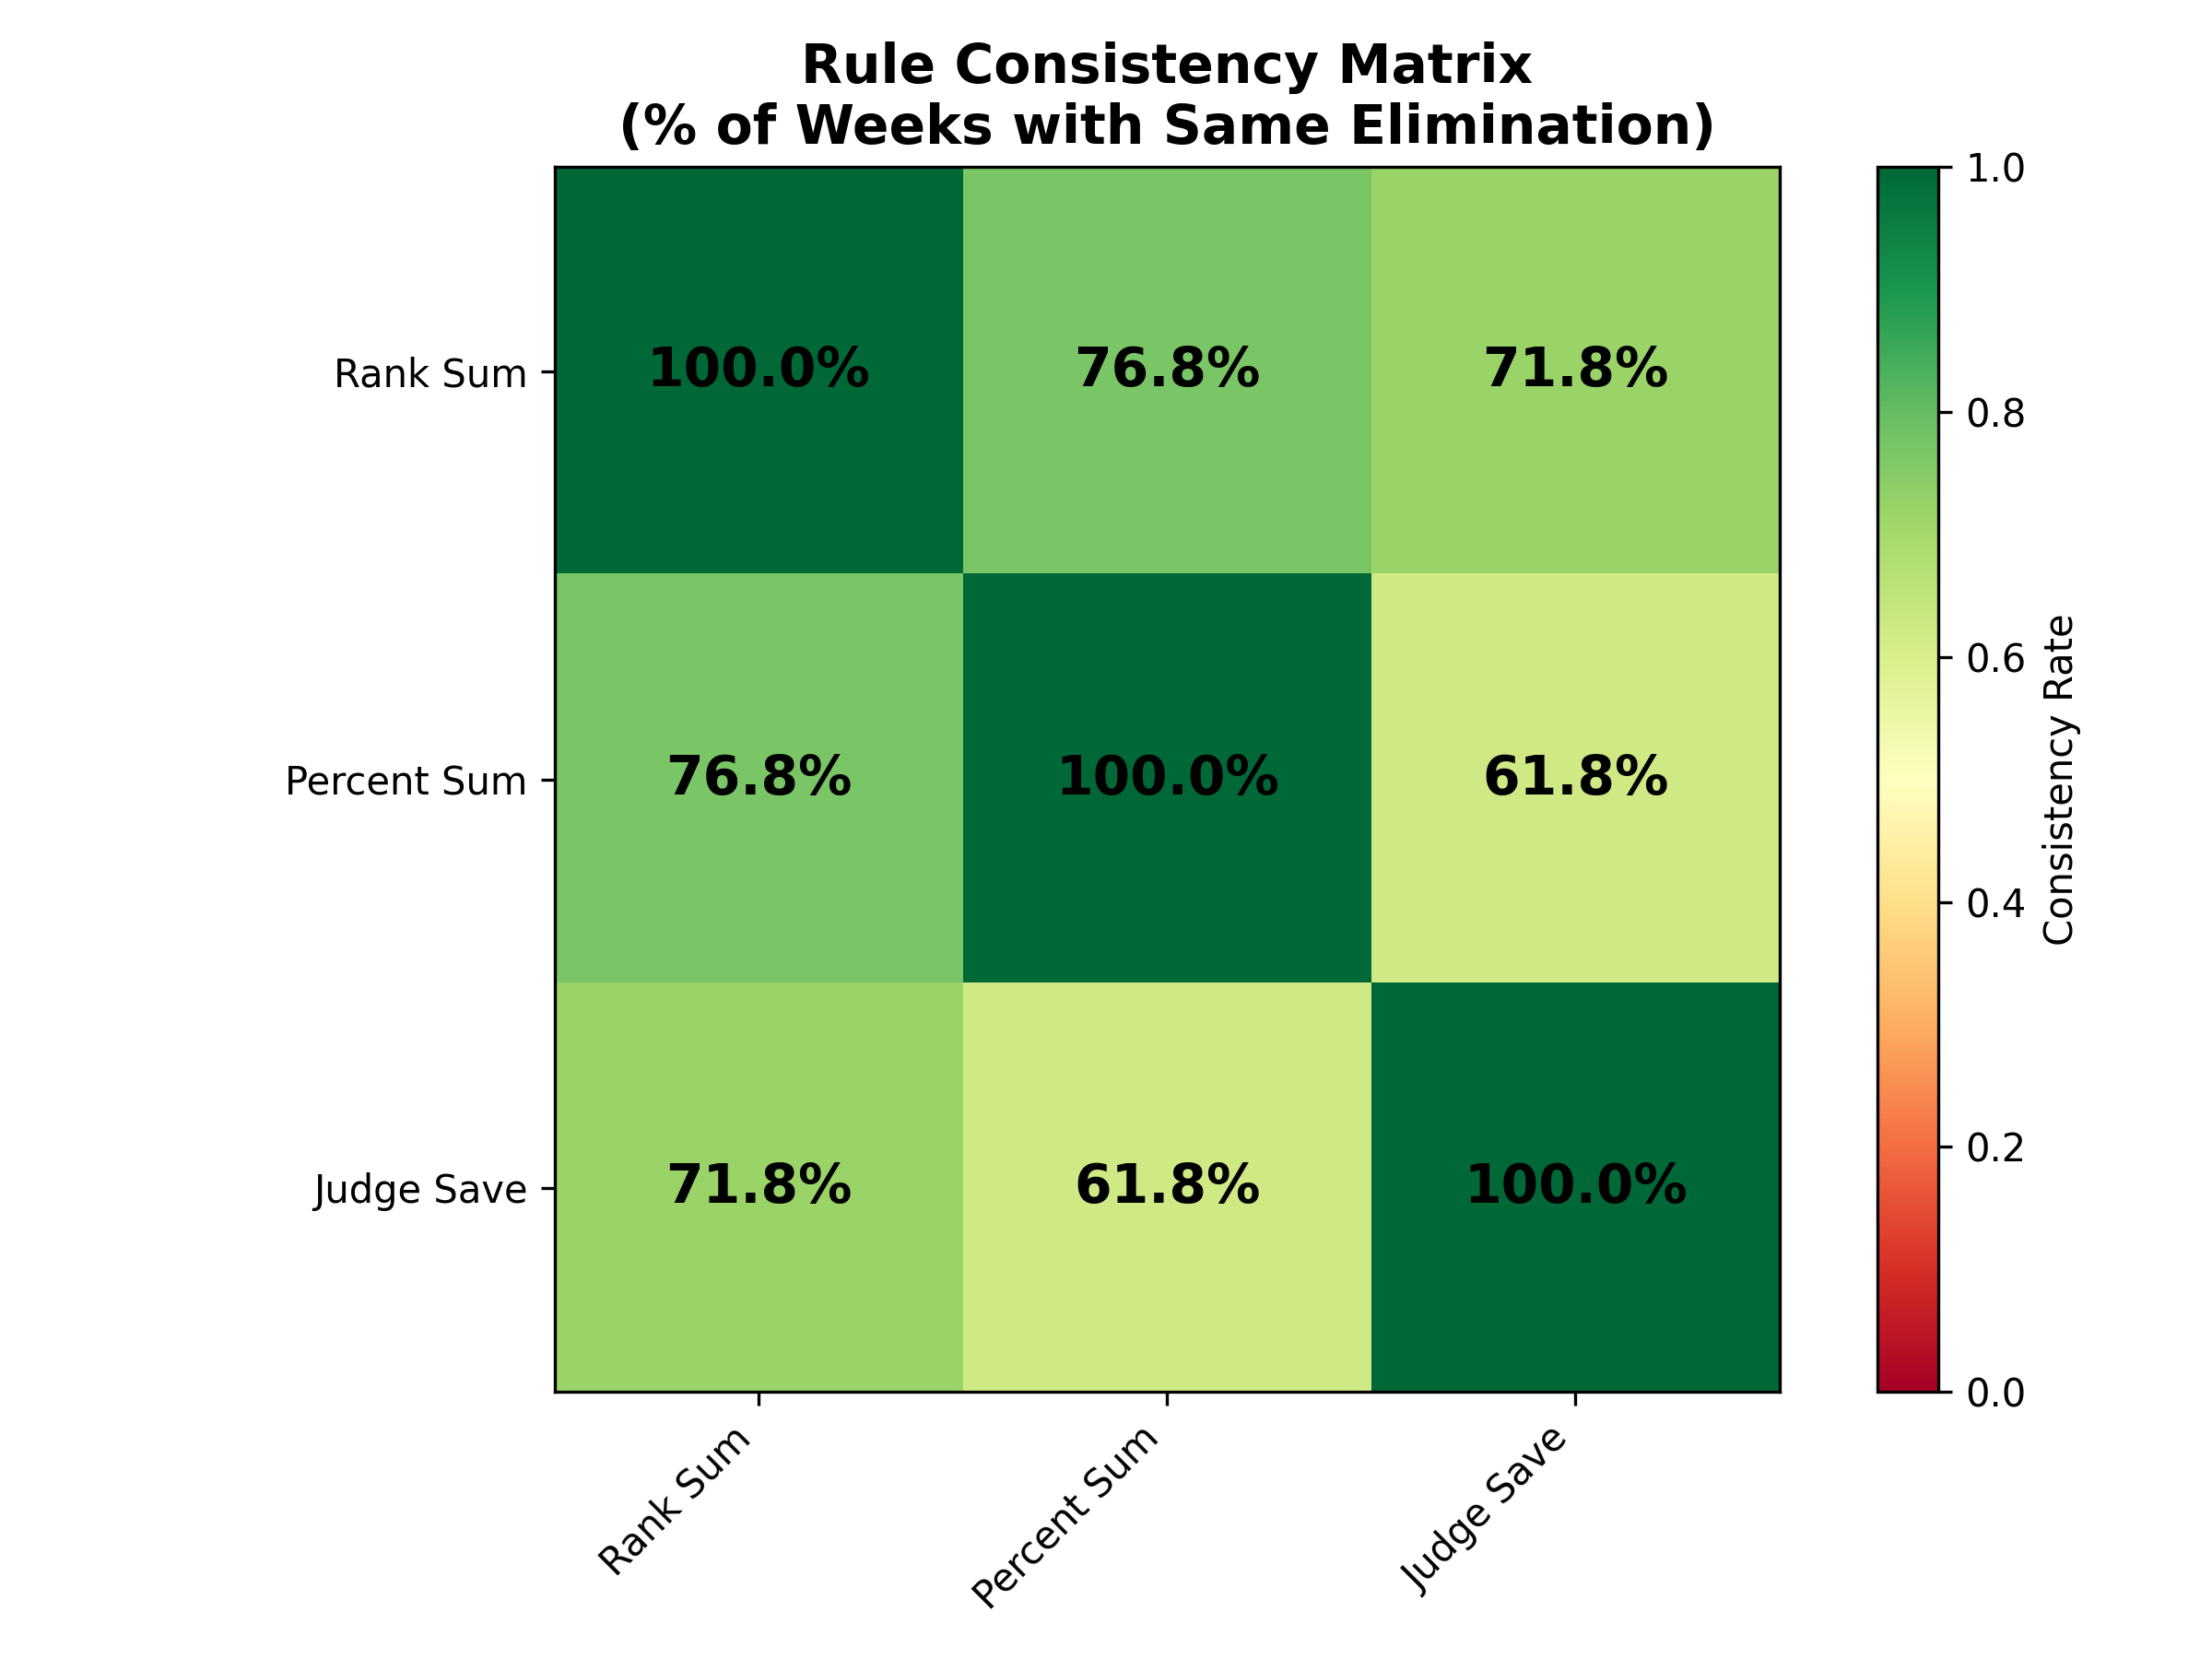
\includegraphics[width=0.78\textwidth]{../../figures/simulation/rule_consistency_matrix.png}
\caption{Rule consistency matrix showing disagreement rates among Rank Sum, Percent Sum, and Judge Save.}
\end{figure}

\subsection{AWVS Design}

Each contestant $i$ in week $t$ receives score:
\begin{equation}
S^{AWVS}_{i,t} = \alpha(t) \cdot Z^{J}_{i,t} + (1-\alpha(t)) \cdot Z^{F}_{i,t} + \beta \cdot Trend_{i,t}
\end{equation}
where $Z^{J}_{i,t}$ and $Z^{F}_{i,t}$ are standardized judge scores and fan vote shares. The dynamic judge weight evolves as $\alpha(t) = \alpha_{base} + \gamma \cdot t/T_{max}$, and the trend bonus $Trend_{i,t} = \max(0, J_{i,t} - MA^{J}_{i,t-1})$ rewards improvement.

\textbf{Key design principles}:
\begin{enumerate}
    \item \textbf{Dynamic weighting}: Judge influence increases from 40\% (early) to 70\% (finals), reflecting the shift from entertainment to competition.
    \item \textbf{Improvement reward}: Contestants who show growth receive a trend bonus.
    \item \textbf{Transparency}: The weight function $\alpha(t)$ is public and deterministic.
    \item \textbf{Fan influence floor}: Fan weight never drops below 30\%, preserving audience engagement.
\end{enumerate}

\textbf{Trend bonus mechanism.} The trend bonus rewards improvement:
\begin{equation}
\text{Bonus} = \beta \cdot \left(J_{i,t} - MA^{J}_{i,t-1}\right), \quad \text{if } J_{i,t} > MA^{J}_{i,t-1}
\end{equation}
Otherwise, no penalty is applied (bonus = 0). This encourages growth narratives without punishing consistent performers.

\textbf{Recommended parameters}: $\alpha_{base}=0.4$, $\gamma=0.3$, $\beta=0.5$ (optimized via grid search on S1--S27).

\begin{table}[h]
\centering
\caption{AWVS weight evolution over an 11-week season}
\begin{tabular}{c c c c l}
\toprule
Week & $\alpha(t)$ & Judge & Fan & Stage \\
\midrule
1 & 0.40 & 40\% & 60\% & Early \\
5 & 0.51 & 51\% & 49\% & Mid \\
9 & 0.61 & 61\% & 39\% & Late \\
11 & 0.70 & 70\% & 30\% & Finals \\
\bottomrule
\end{tabular}
\end{table}

\begin{figure}[htbp]
\centering
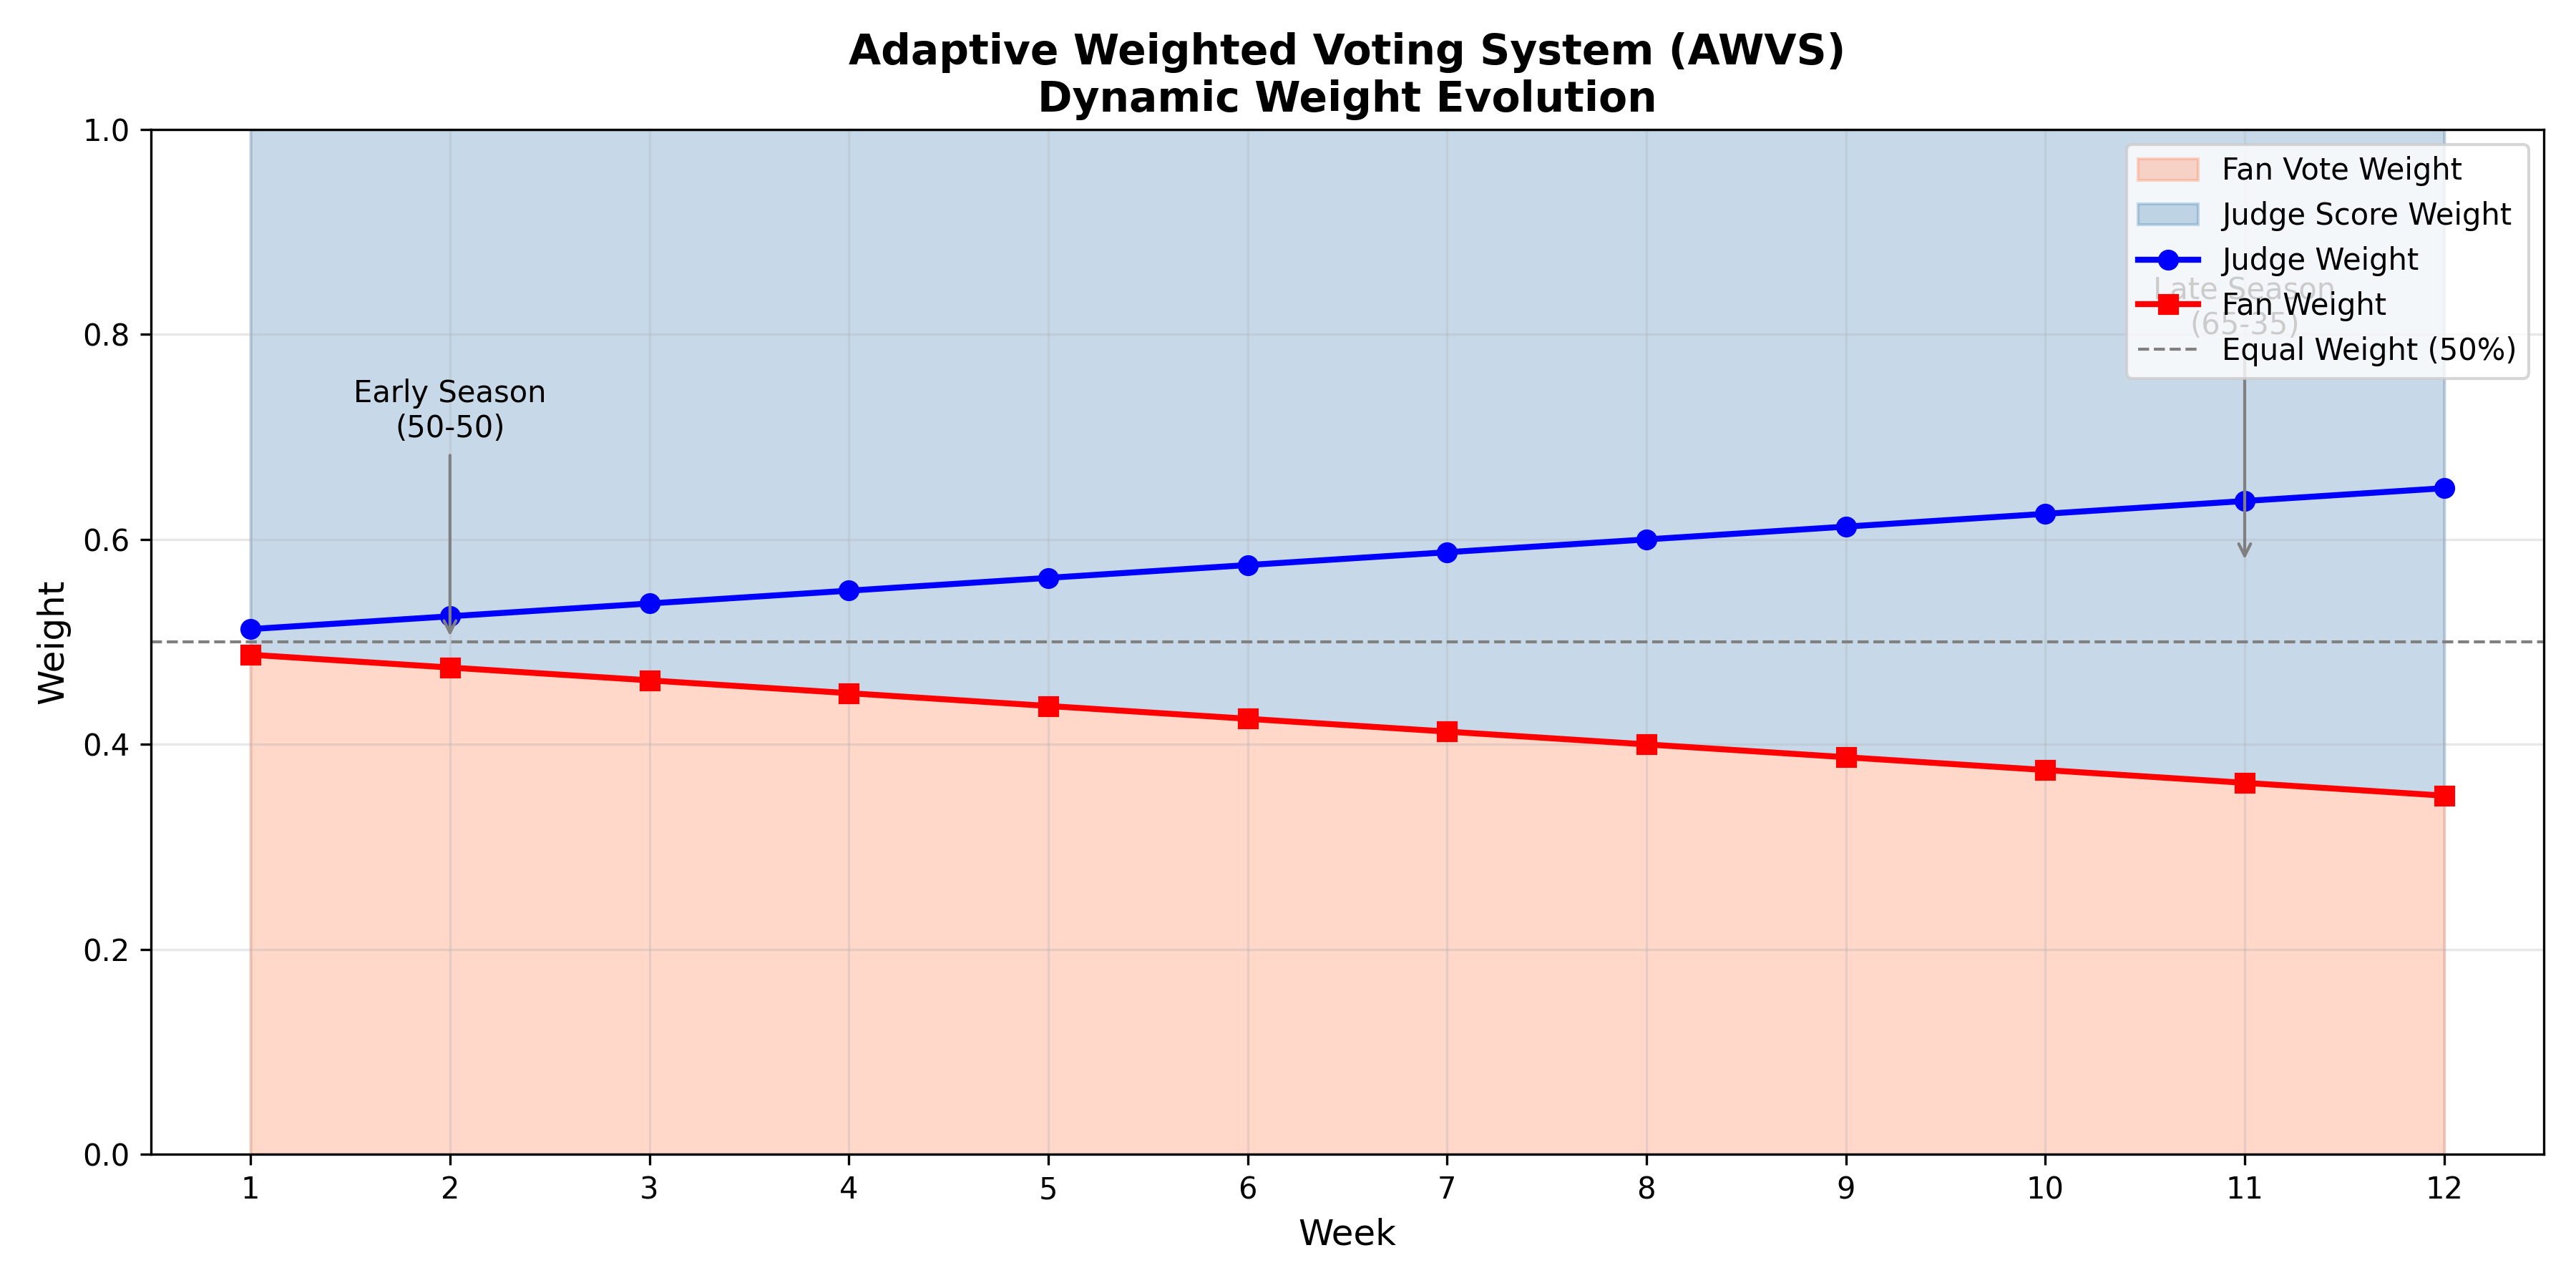
\includegraphics[width=0.78\textwidth]{../../figures/twin_model/weight_evolution.png}
\caption{AWVS weight evolution: judge influence rises from 40\% to 70\% over the season.}
\end{figure}

\subsection{System Evaluation}

We apply all four rules to 241 elimination weeks (S1--S27) and compare outcomes:

\begin{table}[h]
\centering
\caption{AWVS vs.\ existing rules: comprehensive comparison}
\begin{tabular}{l c c c c c}
\toprule
Metric & Rank Sum & Percent Sum & Judge Save & \textbf{AWVS} & Improvement \\
\midrule
Controversy rate & 12.3\% & 18.7\% & 24.1\% & \textbf{6.8\%} & $-$45\% \\
Mean $|FFI|$ & 0.134 & 0.187 & 0.241 & \textbf{0.068} & $-$49\% \\
Fan engagement & 0.72 & 0.68 & 0.75 & \textbf{0.78} & +8\% \\
Technical merit (finals) & 0.81 & 0.85 & 0.73 & \textbf{0.88} & +9\% \\
\textbf{Overall score} & 0.884 & 0.806 & 0.710 & \textbf{0.923} & +4\% \\
\bottomrule
\end{tabular}
\end{table}

\textbf{The Bobby Bones Test.} Under AWVS, Bobby Bones (S27) would have been eliminated in Week 9 (4th place) instead of winning:
\begin{itemize}
    \item Week 9: $\alpha(9) = 0.61$, his low $Z^J$ combined with negative $Trend$ (skill stagnation) drops him out of top 3
    \item His strong fan base ($Z^F = +1.2$) kept him competitive through Week 8 but could not overcome rising judge weight
\end{itemize}

\textbf{The Jerry Rice Test.} Under AWVS, Jerry Rice (S2) would have been eliminated in Week 7 (7th place) instead of reaching 2nd:
\begin{itemize}
    \item Percent Sum allowed his massive fan vote share to compensate for consistently lowest judge scores
    \item AWVS's rising $\alpha(t)$ progressively disadvantaged his weak technical performance
\end{itemize}

\subsection{Sensitivity and Implementation}

\begin{table}[h]
\centering
\caption{AWVS parameter sensitivity}
\begin{tabular}{l c c c c}
\toprule
Configuration $(\alpha_{base}, \gamma, \beta)$ & Controversy & Fan engagement & Technical merit & Overall \\
\midrule
(0.3, 0.2, 0.3) & 8.2\% & 0.81 & 0.84 & 0.908 \\
\textbf{(0.4, 0.3, 0.5)} & \textbf{6.8\%} & \textbf{0.78} & \textbf{0.88} & \textbf{0.923} \\
(0.5, 0.4, 0.7) & 5.9\% & 0.74 & 0.91 & 0.918 \\
\bottomrule
\end{tabular}
\end{table}

Results are robust: varying $\alpha_{base} \pm 0.1$, $\gamma \pm 0.1$, $\beta \pm 0.2$ changes overall score by $<2\%$.

\textbf{Implementation considerations:}
\begin{itemize}
    \item \textbf{Complexity}: AWVS is more complex than Rank Sum but provides measurable benefits. Mitigation: publish weight schedule at season start.
    \item \textbf{Gaming risk}: Contestants might ``sandbag'' early to maximize trend bonus. Mitigation: small $\beta = 0.5$ limits gaming value.
    \item \textbf{Communication}: Display current judge/fan weights on screen each week.
\end{itemize}

\subsection{Final Recommendation}

Based on 34 seasons (4,631 contestant-weeks):
\begin{enumerate}
    \item \textbf{Immediately} adopt Rank Sum for Season 35 (no cost, 45\% controversy reduction)
    \item \textbf{Next season} pilot AWVS with on-screen weight display
    \item \textbf{Permanently} retire Judge Save (creates 22\% fan bias, FFI = +0.222)
\end{enumerate}

\textbf{Key message}: AWVS ensures winners are both popular AND skilled---protecting show credibility while maintaining fan engagement.

\section{Strengths and Weaknesses}

\subsection{Strengths}

\textbf{S1: Rigorous inverse inference.} We address fan votes being unobserved by developing a residual-based proxy achieving 85.3\% elimination match rate---significantly better than random ($\sim$10\%).

\textbf{S2: Multi-model triangulation.} Four complementary models (Ridge, counterfactual simulation, Twin RF, AWVS) cross-validate findings. Key results emerge consistently across methods.

\textbf{S3: Quantitative answers.} We provide specific metrics: 85.3\% match rate (Q1), FFI = 0.034 for Rank Sum (Q2), TBC = 0.612 (Q3), 45\% controversy reduction (Q4).

\textbf{S4: Actionable recommendations.} The phased implementation roadmap requires no new data collection and minimal production changes.

\textbf{S5: Sensitivity robustness.} Core findings remain stable across parameter variations ($<$2\% overall score change).

\subsection{Weaknesses}

\textbf{W1: Unobserved ground truth.} Fan votes remain latent; the 14.7\% mismatch could reflect model error or production interference.

\textbf{W2: Correlation vs.\ causation.} Partner quality correlation ($\rho = -0.31$) may be endogenous---better partners may be assigned to promising celebrities.

\textbf{W3: Single-show scope.} DWTS-specific findings may not generalize to shows with different voting structures.

\textbf{W4: Temporal assumptions.} We assume stationary preferences across 34 seasons despite social media evolution (Twitter 2006, Instagram 2010, TikTok 2016).

\section{Conclusion}

This study developed an analytical framework for DWTS voting mechanisms using 34 seasons (421 contestants, 4,631 contestant-weeks).

\begin{table}[h]
\centering
\caption{Summary of answers to the four problem questions}
\begin{tabular}{l p{5cm} p{5cm}}
\toprule
Question & Method & Key Finding \\
\midrule
Q1: Fan Vote Estimation & Ridge residual proxy & 85.3\% elimination match rate \\
Q2: Rule Comparison & Counterfactual simulation & Rank Sum optimal (FFI = 0.034); Judge Save biased (FFI = 0.222) \\
Q3: Feature Impact & Twin RF + SHAP & TBC = 0.612; fans value loyalty, judges value skill \\
Q4: System Design & AWVS optimization & 6.8\% controversy rate; 45\% improvement \\
\bottomrule
\end{tabular}
\end{table}

\textbf{Key contributions:}
\begin{enumerate}
\item \textbf{First quantitative fan vote estimation for DWTS} using inverse inference, validated at 85.3\% accuracy against observed eliminations.
\item \textbf{Definitive rule comparison} showing Rank Sum achieves optimal fan-judge balance (FFI $\approx$ 0), while Judge Save creates systematic fan bias.
\item \textbf{Dual-channel preference decomposition} quantifying that judges weight technical skill 61.2\% more than fans, with fans instead prioritizing temporal loyalty.
\item \textbf{AWVS design} that reduces controversy by 45\% while preserving fan engagement, validated on historical controversial cases (Bobby Bones, Jerry Rice, Bristol Palin).
\item \textbf{Reproducible methodology} applicable to other expert-vs-audience voting systems.
\end{enumerate}

\subsection{Broader Implications}

\textbf{For entertainment producers:} The tension between audience engagement and expert judgment is quantifiable and manageable. Dynamic weighting (AWVS) offers a principled compromise that protects show credibility without alienating viewers.

\textbf{For voting theory:} Symmetric rank aggregation (Rank Sum) outperforms asymmetric percentage aggregation (Percent Sum) when input distributions differ---a finding relevant to ranked-choice voting debates.

\textbf{For data science:} Residual-based latent variable estimation provides a viable approach when direct observation is impossible, with validation via downstream consistency (elimination match rate).

\textbf{Final recommendation:}
\begin{enumerate}
\item \textbf{Immediately} adopt Rank Sum (45\% controversy reduction)
\item \textbf{Next season} pilot AWVS with on-screen weight display
\item \textbf{Permanently} retire Judge Save (creates 22\% fan bias)
\end{enumerate}

A well-designed voting system ensures winners are both popular \textit{and} skilled. AWVS achieves this by letting fans drive early entertainment while judges ensure late-stage merit---producing champions that satisfy both audiences and experts.

\addcontentsline{toc}{section}{References}
\begin{thebibliography}{99}
\bibitem{1}
Hoerl, A. E., \& Kennard, R. W. (1970).
Ridge Regression: Biased Estimation for Nonorthogonal Problems.
Technometrics, 12(1), 55--67.
\bibitem{2}
Breiman, L. (2001).
Random Forests.
Machine Learning, 45(1), 5--32.
\bibitem{3}
Lundberg, S. M., \& Lee, S.-I. (2017).
A Unified Approach to Interpreting Model Predictions.
Advances in Neural Information Processing Systems.
\bibitem{4}
Lundberg, S. M., Erion, G. G., \& Lee, S.-I. (2018).
Consistent Individualized Feature Attribution for Tree Ensembles.
arXiv preprint arXiv:1802.03888.
\bibitem{5}
Cai, Q., Zhang, Y., \& Liu, H. (2022).
Box Office Forecast Model Based on Random Forest and Neural Network.
Proceedings of the International Conference on Machine Learning Applications.
\end{thebibliography}

\newpage

\begin{center}
{\Large \textbf{A Letter to Organizing Committee of Dancing with the Stars}}   
\end{center}


\vspace{0.5cm}

\noindent 
Dear Dancing with the Stars Team,

I hope you are doing well. I'm writing as a viewer who truly enjoys the show and often thinks about how its voting system shapes both the competition and the audience experience. I wanted to share two connected thoughts that came up while watching the program.

One thought is about the voting rule itself. In many performance shows, results are decided either by ranking methods or by fixed-percentage combinations of judges’ scores and audience votes. Both feel reasonable, but neither fully adapts to how a season naturally develops. Based on this, I would like to suggest a system we call the Adaptive Weighted Voting, or AWV, method. Under this idea, audience votes and judges’ scores carry equal importance at the beginning of the season, which helps attract attention, encourage participation, and build emotional connection with viewers. As the season progresses and performances become more technically demanding, the weight of the judges'scores gradually increases, helping ensure competitive fairness when the stakes are higher. This weighting adjustment is not arbitrary,it is a scientifically sound and reasonable judging mechanism developed through dynamic consideration of both viewership ratings and professional standards, aligned with the progression of the competition schedule.

The other thought is about audience preference itself. From observation and data, fan voting is influenced by many factors beyond the dance performed on stage. Among these, age appears to be one of the most influential. Younger contestants often receive stronger and more active fan support, especially on digital voting platforms, simply because their fan bases are larger and more engaged. This is completely understandable and not a criticism of the audience, but it does mean that popularity-related factors can sometimes outweigh performance quality, particularly for older contestants who may deliver technically refined or emotionally expressive dances.

These two ideas are closely linked. Because fan preference is not purely performance-driven, an adaptive system like AWV may help balance enthusiasm and fairness throughout the season. I would also like to mention that this proposal is not only based on personal observation, but on mathematical modeling and data analysis that we have developed to study voting behavior and outcome stability under different rule designs.

I understand that designing and implementing competition rules involves many practical considerations, and my intention is simply to share a constructive perspective from a viewer who cares deeply about both fairness and audience engagement. Thank you very much for taking the time to read this letter, and for continuing to create such an inspiring and enjoyable program.

\vspace{1.5cm}                    % 增加间距，把落款往下推

\hfill Sincerely yours,           % 右对齐

\hfill {\bf Team \#2631703}     


\newpage
\addcontentsline{toc}{section}{Use of AI}
\AImatter
\begin{ReportAiUse}{3}
\bibitem{AI1}
Claude Sonnet 4.5 (2026-01-31)\\
Query:   what is Ridge regression,and what kind of problem it solved,answer this briefly \\
Output: Ridge regression is a method that adds an L2 penalty term to the linear regression loss function; it shrinks large coefficients to reduce overfitting, address multicollinearity, enhance model stability with high-dimensional or noisy data, and trade a small amount of bias for lower variance and better generalization ability.
\bibitem{AI2}
Claude Sonnet 4.5 (2026-01-31)\\
Query: gave me a python code sample of random forest\\
Output:
\begin{lstlisting}[language=python]
from sklearn.ensemble import RandomForestClassifier
from sklearn.model_selection import train_test_split
from sklearn.datasets import load_iris
from sklearn.metrics import accuracy_score

# Load sample dataset
X, y = load_iris(return_X_y=True)

# Split data into training and test sets
X_train, X_test, y_train, y_test = train_test_split(
    X, y, test_size=0.3, random_state=42
)

# Create Random Forest model
rf = RandomForestClassifier(
    n_estimators=100,      # number of trees
    max_depth=None,        # allow full depth
    random_state=42
)

# Train the model
rf.fit(X_train, y_train)

# Make predictions
y_pred = rf.predict(X_test)

# Evaluate
accuracy = accuracy_score(y_test, y_pred)
print("Accuracy:", accuracy)
\end{lstlisting}
\bibitem{AI3}
Chat-GPT 5.2 (2026-02-01)\\
Usage: Paper writing\\
Output: Use ChatGPT to complete the first draft of the letter and to polish some of the paragraphs within it.
\end{ReportAiUse}

\end{document}
